% =============================================================================
% main.tex — preliminary brief for the advisor, written as the skeleton of the paper.
%
% Build (from the Writing folder):
%   python3 scripts/make_tables.py      (or: uv run python Writing/scripts/make_tables.py from the project root)
%   latexmk -pdf main.tex
%
% Tables are generated from the CSV results (tables/*.tex, do not edit by hand).
% Figures are read directly from ../empirics/results/figures/.
% Numbers quoted in the TEXT refer to the run of 2026-10-22 16:45 and must be
% checked by hand after a new run (search for "% NUMBERS" comments).
% Paragraphs marked [PAPER] are placeholders for the later paper version.
% =============================================================================
\documentclass[11pt,a4paper]{article}

\usepackage[T1]{fontenc}
\usepackage[utf8]{inputenc}
\usepackage{lmodern}
\usepackage{microtype}
\usepackage[margin=2.5cm]{geometry}
\usepackage{setspace}
\usepackage{amsmath,amssymb}
\usepackage{graphicx}
\usepackage{booktabs,threeparttable,makecell}
\usepackage{caption}
\captionsetup{font=small,labelfont=bf}
\usepackage{float}
\usepackage{enumitem}
\setlist{itemsep=2pt,topsep=4pt}
\usepackage{xcolor}
\usepackage[authoryear,round]{natbib}
\usepackage[colorlinks=true,linkcolor=blue!50!black,citecolor=blue!50!black,urlcolor=blue!50!black]{hyperref}
\usepackage{mdframed}

\graphicspath{{../empirics/results/figures/}{../empirics/results/figures/descriptives/}}

% Notes to the advisor / to ourselves; set \showtodostrue to \showtodosfalse to hide them in the paper
\newif\ifshowtodos \showtodostrue
\newcommand{\todo}[1]{\ifshowtodos{\color{red!70!black}\textbf{[To do:} #1\textbf{]}}\fi}
\newcommand{\paperonly}[1]{\ifshowtodos{\color{gray}\textit{[Paper: #1]}}\fi}

\newcommand{\Sanc}{S_{it}}
\newcommand{\Viol}{V_{it}}

\title{Do Sanctions Break the Cycle of Violence?\\[4pt]
\large Panel-VAR evidence on sanctions and organized violence, 1989--2019\\[2pt]
\normalsize Preliminary results --- brief for discussion}
\author{}
\date{}

\begin{document}
\maketitle
\onehalfspacing

% =============================================================================
\begin{mdframed}[linewidth=0.6pt,innerleftmargin=10pt,innerrightmargin=10pt]
\textbf{Summary for the meeting.}
% NUMBERS: Table 1, Table 4, Table 5, gdelt tables, tab:controls, tab:yugoslavia (run 2026-10-23 16:50)
\begin{enumerate}[leftmargin=*]
\item \textbf{Design.} A panel version of \citet{jaeger2008}: two reaction functions (new sanctions on past
  violence; violence on past new sanctions) forming a bivariate VAR(2) with state and year fixed effects, for
  197 states, 1989--2019. Sanctions are \emph{new} cases from the GSDB, violence is UCDP organized violence. Same
  outputs as the original: Granger tests, lag-structure grid, response functions, cumulative impulse responses.
\item \textbf{Senders react to violence.} Past violence predicts new sanctions (Granger $p=0.007$ incidence,
  $p=0.026$ levels, state and year FE only); a conflict year raises the number of new-sanction years over the next
  decade by 0.09--0.16 (11 of 12 IRF versions significant). The effect weakens when GDP growth is controlled for,
  which is plausibly a bad control.
\item \textbf{Violence reacts to sanctions with a two-year lag --- in deaths, not in conflict incidence.} Two
  years after a new sanction case, log deaths per 100,000 are lower (sum of the lag coefficients $-0.035$ with
  fixed effects only, $p=0.028$; $-0.050$ with controls, $p=0.018$). This holds with every set of controls, with the
  jackknife, GMM, and PPML on winsorised deaths ($-11$ to $-16$\%); the cumulative impulse response is negative but
  not significant. The 3.5 percentage-point lower conflict probability reported earlier appears only when the
  stock of sanctions in force in $t-1$ is controlled for. That stock contains the tested sanction lags, so this
  result is mechanical (Table~\ref{tab:controls}). If sanctions may affect violence within the same year, the
  cumulative response turns positive.
\item \textbf{Robustness.} Stationarity, stability and residual diagnostics are fine. GMM, PPML and raw (capped)
  deaths confirm the negative $t-2$ effect on deaths. All states, including the successor states of Yugoslavia,
  are in the main sample (only the Yugoslavia dummy was dropped from the controls); when these eight states are
  excluded as a robustness check, the effect is weaker ($p=0.08$ with fixed effects only, Table~\ref{tab:yugoslavia}). With GDELT (media-reported violence) the incidence estimate is
  negative but not significant, low-level violence \emph{rises} after sanctions, and senders do not
  react to GDELT violence.
\end{enumerate}
\end{mdframed}

% =============================================================================
\section{Introduction}
\label{sec:intro}

Sanctions are the most frequently used coercive tool short of force, and a large share of them is imposed in
response to political violence: to end civil wars, stop atrocities or punish repression. Whether they achieve
this, or instead feed a cycle in which violence triggers sanctions and sanctions trigger more violence, is an
open empirical question.

This project brings the empirical framework of \citet{jaeger2008} --- built to ask whether one side's violence
predicts the other side's violence in the Second Intifada --- to a cross-country panel: do senders react to
violence in a target state, and does violence react to new sanctions? We estimate both reaction functions
jointly as a panel VAR on 197 states over 1989--2019, using the Global Sanctions Data Base
\citep{felbermayr2020,yalcin2024} and UCDP data on organized violence \citep{davies2026}.

\paragraph{Preliminary contribution.}
\begin{itemize}[leftmargin=*]
\item The first cross-country panel VAR of \emph{sanctions} and \emph{fatal violence}. The closest work,
  \citet{dizaji2024}, uses arms-import shocks as a proxy for embargoes and an expert risk index for conflict in
  48 selected countries.
\item A design that separates the two directions of the relationship, which the cross-sectional sanctions
  literature typically does not.
\item Inference that takes the short-$T$ panel seriously: Nickell-bias corrections, GMM, cluster bootstrap.
\end{itemize}
\paperonly{motivation with recent examples (Myanmar 2021, Russia 2014/2022, Sudan); policy relevance; roadmap.}

% =============================================================================
\section{Related literature}
\label{sec:literature}

\paragraph{Sanctions and political violence.}
Most cross-national studies relate the \emph{presence} of sanctions to an outcome of the target state. Economic
sanctions are associated with more state repression \citep{wood2008}, worse physical-integrity rights
\citep{peksen2009} and declining democracy \citep{peksen2010}. For armed conflict, the evidence is mixed.
\citet{hultman2017} study African civil conflicts 1989--2005 and find that threatened and imposed economic
sanctions tend to intensify fighting, while imposed arms embargoes reduce it. \citet{escribafolch2010} finds that
sanctions are associated with shorter civil wars, with institutional sanctions favouring negotiated settlements,
whereas \citet{lektzian2016} argue that sanctions on their own rarely shorten civil conflicts and help mainly as
part of a broader response including military intervention. At the sub-national level, \citet{urtuzuastigui2024}
find that targeted sanctions on armed actors increase violence against civilians (resource substitution);
\citet{stork2020} reports a similar pattern for UN sanctions on rebel groups. The literature on targeted
sanctions \citep{drezner2011,biersteker2016} and on sanction success \citep{hufbauer2007} provides the
institutional background. A common limitation is the treatment of sanctions as exogenous, although they are often
imposed \emph{because of} violence: this reverse direction is exactly what a VAR models.

\paragraph{Cycles of violence and VARs.}
\citet{jaeger2008} estimate two reaction functions with daily fatality data and show that Palestinian fatalities
Granger-cause Israeli responses but not the reverse; \citet{asali2017} revisit the result with nonlinear VARs.
The closest cross-country application is \citet{dizaji2024}, a panel VAR in which negative shocks to arms imports
(a proxy for embargoes) are followed by lower military spending but \emph{more} internal conflict; their
methodological template is \citet{dizaji2023}. Their design differs from ours in four respects that matter: no
sanctions data, an expert risk index instead of fatalities, 48 selected countries, and no treatment of the
Nickell bias or of year effects.

\paragraph{Methods.}
Panel VARs go back to \citet{holtzeakin1988}; the GMM workflow we use as a robustness check follows
\citet{love2006} and \citet{abrigo2016}. With $T\approx 30$, fixed-effects estimates of dynamic models are biased
\citep{nickell1981}; we use the half-panel jackknife \citep{dhaene2015}, which \citet{juodis2021} combine with a
pooled Granger test for heterogeneous panels \citep[implemented by][]{xiao2023}; alternatives are
\citet{dumitrescu2012} and, under cross-sectional dependence, \citet{nazlioglu2024}. For impulse responses, VARs
and local projections \citep{jorda2005} estimate the same object \citep{plagborg2021}, with a bias--variance
trade-off \citep{li2024}; panel local projections have their own Nickell bias \citep{mei2026}. Event-study
designs with on/off treatments \citep{dube2023,dechaisemartin2026} are a possible extension. Finally,
$\log(1+y)$ effects with many zeros are not percentage effects \citep{chen2024}, which is why we read signs and
significance from the levels specification and magnitudes from the incidence specification.

\todo{literature from the \texttt{papers/} folder is read in full; the political-science entries above are
from abstracts --- read in full before the paper version.}

% =============================================================================
\section{Data}
\label{sec:data}

\paragraph{Sample.} All states of the \citet{gleditsch1999} system with at least ten years of data in 1989--2019:
197 states and 5,932 state-years (four short-lived states excluded). States that are never in conflict (about 90)
or never newly sanctioned (31) are kept: dropping them would select on the outcome.
The panel is built with the \texttt{peacesciencer} framework \citep{miller2022}.

\paragraph{Sanctions.} The Global Sanctions Data Base, release 4 \citep{felbermayr2020,yalcin2024}, covers 1,547
cases 1950--2023. Because the stock of sanctions in force is highly persistent (more than half of all state-years
are under some sanction), the VAR uses the \emph{flow}: $\texttt{new\_sanction}_{it}=1$ if at least one case
against state $i$ begins in year $t$ (incidence), and the number of new cases (levels). The construction
reproduces the GSDB's own counts (e.g.\ 25 new and 38 active cases against Russia in 2022).

\paragraph{Violence.} UCDP organized violence, country-year version 26.1 \citep{davies2026}: deaths in
state-based, non-state and one-sided violence. Incidence: conflict year with at least 25 deaths. Levels:
$\log(1+\text{deaths per }100{,}000)$; the transformation is needed because the top 1\% of state-years account
for 99.9\% of the variance of raw deaths (Rwanda 1994).

\paragraph{Controls} (lagged one year): number of sanction cases in force, GDP per capita growth, V-Dem polyarchy
\citep{vdem2025}.

\paragraph{Yugoslavia dummy (dropped).} GSDB cases against Yugoslavia are attributed to its successor states (see
\texttt{data/README\_yugoslavia.md}), so one case can appear as a new case in several states in the same year.
Earlier versions of this brief therefore also controlled for a dummy equal to one for the successor states of
Yugoslavia in 1991--2016. With state fixed effects, however, this dummy is identified only from the years 2017--2019
in seven of these states (for Yugoslavia/FRY itself it is constant and fully absorbed), years with no new sanction
and no conflict; and a level shift cannot remove cases that are counted in several states at once. It was dropped
from the controls on 23 October 2026. Dropping it leaves the sanctions$\rightarrow$violence tests unchanged
(incidence $\chi^2(2)=7.27$, $p=0.026$; levels $8.08$, $p=0.018$) and moves the violence$\rightarrow$sanctions tests
only slightly (incidence $6.11 \rightarrow 6.22$, levels $2.79 \rightarrow 2.82$; Table~\ref{tab:granger}, Panel A).
The attribution problem itself is addressed in Section~\ref{sec:controls}, which drops the ex-Yugoslav states or
treats them as one cluster (Table~\ref{tab:yugoslavia}).

\paragraph{Alternative violence measure.} GDELT 1.0 \citep{leetaru2013}: media-reported assault, fight and
mass-violence events as a share of all GDELT events in the state-year (1979--2021), which captures violence below
the UCDP threshold.

\begin{table}[htbp]
\centering
\small
\caption{Descriptive statistics, 1989--2019}
\label{tab:descriptives}
\begin{threeparttable}
\begin{tabular}{lrrr}
\toprule
Variable & Mean & SD & $N$ \\
\midrule
New sanction (0/1) & 0.108 & 0.311 & 5,932 \\
Number of new sanction cases & 0.164 & 0.618 & 5,932 \\
Conflict, $\geq$ 25 deaths (0/1) & 0.205 & 0.403 & 5,932 \\
$\log(1 + \text{deaths per 100,000})$ & 0.268 & 0.779 & 5,932 \\
Deaths per 100,000 (raw) & 4.541 & 164.641 & 5,932 \\
Sanction cases in force, $t-1$ & 1.344 & 2.254 & 5,903 \\
GDP per capita growth, $t-1$ & 0.018 & 0.041 & 5,874 \\
V-Dem polyarchy, $t-1$ & 0.498 & 0.272 & 5,234 \\
\bottomrule
\end{tabular}
\begin{tablenotes}[flushleft]\footnotesize
\item \textit{Notes:} State-years of the estimation panel (197 states, 1989--2019). Sanctions: Global Sanctions Data Base (GSDB, release 4), flows of new cases constructed from case start years. Violence: UCDP organized violence, country-year (v26.1). Controls are lagged one year; missing controls are mostly microstates without V-Dem data.
\end{tablenotes}
\end{threeparttable}
\end{table}


\begin{figure}[htbp]
\centering
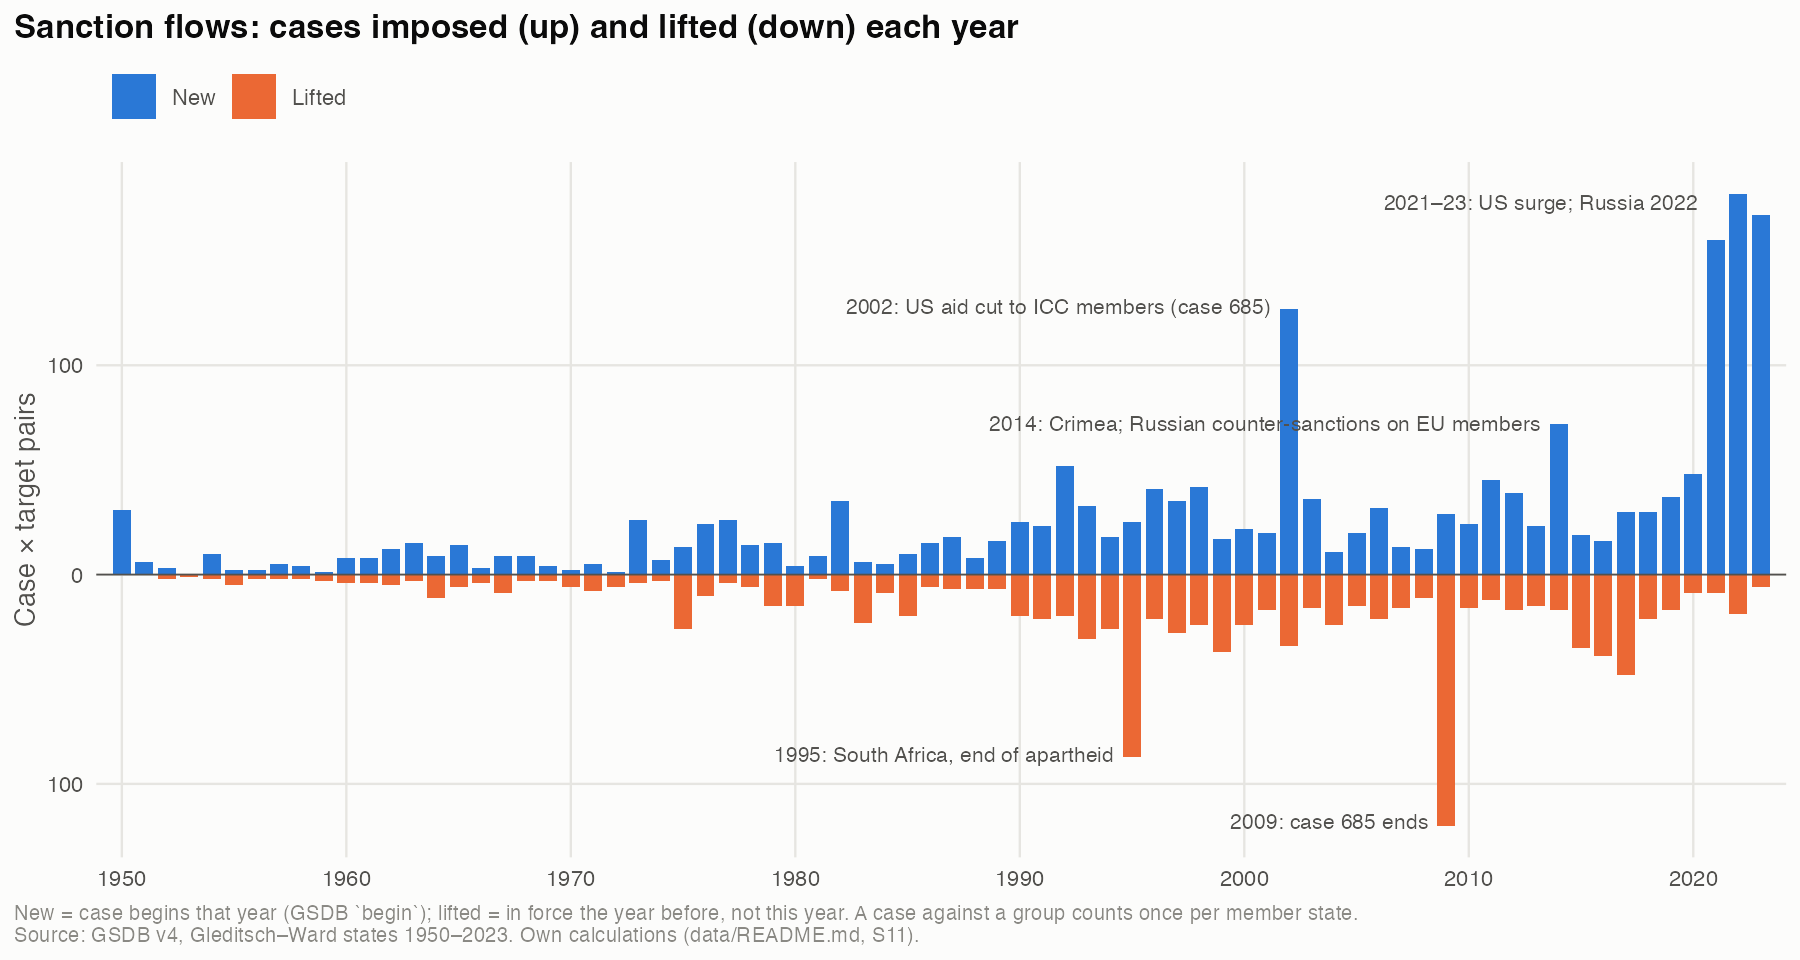
\includegraphics[width=0.85\textwidth]{fig6_new_lifted_cases_per_year.png}
\caption{New and lifted sanction cases per year (GSDB)}
\label{fig:flows}
\end{figure}

\paperonly{data appendix: case-level construction of flows, Yugoslavia attribution, GDELT country assignment;
all decisions are documented in \texttt{data/README.md}.}

% =============================================================================
\section{Empirical strategy}
\label{sec:strategy}

\paragraph{Reaction functions.} Following \citet{jaeger2008}, the two equations are
\begin{align}
\Viol &= \sum_{k=1}^{p} a_k V_{i,t-k} + \sum_{k=1}^{p} b_k S_{i,t-k} + \gamma' X_{i,t-1} + \mu_i + \tau_t + \varepsilon_{it}, \label{eq:violence}\\
\Sanc &= \sum_{k=1}^{p} d_k S_{i,t-k} + \sum_{k=1}^{p} c_k V_{i,t-k} + \delta' X_{i,t-1} + \nu_i + \lambda_t + u_{it}, \label{eq:sender}
\end{align}
with $p=2$, state fixed effects ($\mu_i,\nu_i$), year fixed effects ($\tau_t,\lambda_t$) and lagged controls
$X$. Together they form a bivariate panel VAR. As in the original, each equation is estimated by OLS (linear
probability models in the incidence version); standard errors are clustered by state.

\paragraph{Granger tests.} H$_0$: $b_1=b_2=0$ (sanctions do not predict violence) and H$_0$: $c_1=c_2=0$
(violence does not predict sanctions); Wald $\chi^2(2)$. A rejection means predictive precedence conditional on
the own history and the fixed effects, not causation.

\paragraph{Nickell bias.} With $T\approx 30$ the fixed-effects estimates of dynamic coefficients are biased by
$O(1/T)$ \citep{nickell1981}, which is of the same order as their standard errors. We therefore report
(i) the half-panel jackknife $\tilde\beta = 2\hat\beta - (\hat\beta_{1991-2005}+\hat\beta_{2006-2019})/2$
\citep{dhaene2015,juodis2021}, and (ii) a GMM panel VAR with forward orthogonal deviations and collapsed
instruments \citep{abrigo2016}.

\paragraph{Impulse responses.} The VAR traces the joint dynamics after a one-unit shock (one new sanction / one
conflict year). Annual data leave the within-year ordering open, so we report three identifications: no same-year
effect on the other variable \citep[fn.~12]{jaeger2008}, and the two Cholesky orderings. Confidence bands come
from a country-cluster bootstrap.

\paragraph{Response functions.} The model-free analogue of \citet[Fig.~2]{jaeger2008}: the difference between the
mean outcome $k$ years after an event year and in all other years, raw and net of state and year means.

\paperonly{discussion of identification: what Granger causality can and cannot show here; forward-looking senders;
omitted common drivers.}

% =============================================================================
\section{Results}
\label{sec:results}
% NUMBERS: section 5 (run 2026-10-23 16:50)

\subsection{Granger tests}

Table~\ref{tab:granger} is the panel analogue of \citet[Table 1]{jaeger2008}; the full coefficients are in
Table~\ref{tab:coefficients}.

\textit{Sanctions $\rightarrow$ violence (Panel A).} The lags of new sanctions are jointly significant at the 5\% level in six
of eight FE-OLS and jackknife versions (all eight at 10\%) and in all four GMM versions. The effect sits at $t-2$. In levels, a new sanction case
is followed two years later by fewer deaths per capita (sum $-0.035$ without and $-0.050$ with controls). For
incidence, the sum is negative only with controls ($-0.035$, i.e.\ a 3.5 percentage-point lower conflict
probability); without controls it is close to zero because the $t-1$ coefficient turns slightly positive.
Table~\ref{tab:controls} (Section~\ref{sec:controls}) shows which control is responsible: the stock of sanctions
in force in $t-1$, which mechanically contains the new cases of $t-1$ and $t-2$. With the stock dated $t-3$, or with
GDP growth or democracy alone, the incidence sum is again close to zero on the same sample. The incidence result
should therefore not be read as an effect of sanctions; the levels result holds in every version.

\textit{Violence $\rightarrow$ sanctions (Panel B).} Past violence predicts new sanctions in the specifications
with fixed effects only (OLS and jackknife). With controls the test weakens, mainly through GDP growth: conflict
lowers growth, and low growth predicts sanctions, so growth is plausibly a channel rather than a confounder. On a
common sample, the incidence test is significant with every control and the levels test is lost only with GDP
growth (Table~\ref{tab:controls}). In
GMM the incidence version is insignificant, but the GMM incidence models fail or nearly fail the Hansen test
(Table~\ref{tab:gmm}).

\begin{table}[htbp]
\centering
\footnotesize
\caption{Granger causality tests: panel version of Jaeger and Paserman (2008), Table 1}
\label{tab:granger}
\begin{threeparttable}
\begin{tabular}{lcccccc}
\toprule
 & \multicolumn{2}{c}{FE-OLS} & \multicolumn{2}{c}{Half-panel jackknife} & \multicolumn{2}{c}{GMM} \\
\cmidrule(lr){2-3}\cmidrule(lr){4-5}\cmidrule(lr){6-7}
 & Controls & FE only & Controls & FE only & Controls & FE only \\
\midrule
\multicolumn{7}{l}{\textit{Panel A: Sanctions $\rightarrow$ violence}} \\
\quad Incidence & 7.27$^{**}$ & 5.01$^{*}$ & 7.87$^{**}$ & 4.85$^{*}$ & 6.26$^{**}$ & 6.17$^{**}$ \\
\quad  & (0.026) & (0.082) & (0.020) & (0.088) & (0.044) & (0.046) \\
\quad  & [$-$0.035] & [0.002] & [$-$0.040] & [0.006] & [$-$0.029] & [0.002] \\
\quad Levels & 8.08$^{**}$ & 7.14$^{**}$ & 7.84$^{**}$ & 6.18$^{**}$ & 11.61$^{***}$ & 7.48$^{**}$ \\
\quad  & (0.018) & (0.028) & (0.020) & (0.045) & (0.003) & (0.024) \\
\quad  & [$-$0.050] & [$-$0.035] & [$-$0.054] & [$-$0.035] & [$-$0.068] & [$-$0.041] \\
\midrule
\multicolumn{7}{l}{\textit{Panel B: Violence $\rightarrow$ sanctions}} \\
\quad Incidence & 6.11$^{**}$ & 9.86$^{***}$ & 3.80 & 11.29$^{***}$ & 0.56 & 0.56 \\
\quad  & (0.047) & (0.007) & (0.149) & (0.004) & (0.756) & (0.758) \\
\quad  & [0.055] & [0.070] & [0.044] & [0.075] & [0.021] & [0.023] \\
\quad Levels & 2.79 & 7.30$^{**}$ & 3.77 & 22.78$^{***}$ & 3.01 & 7.77$^{**}$ \\
\quad  & (0.248) & (0.026) & (0.152) & ($<$0.001) & (0.222) & (0.021) \\
\quad  & [0.030] & [0.045] & [0.037] & [0.092] & [0.035] & [0.074] \\
\midrule
Observations & 4,913 & 5,538 & 4,913 & 5,538 & 4,739 & 5,341 \\
States & 174 & 197 & 174 & 197 & 174 & 197 \\
\bottomrule
\end{tabular}
\begin{tablenotes}[flushleft]\footnotesize
\item \textit{Notes:} Wald $\chi^2(2)$ statistic for the joint significance of the two lags of the other variable in a bivariate panel VAR(2) with state and year fixed effects; $p$-value in parentheses; sum of the two lag coefficients in brackets (negative in Panel A = less violence after new sanctions). Incidence: new sanction (0/1) and conflict with $\geq$ 25 deaths (0/1), linear probability models. Levels: number of new cases and $\log(1+$deaths per 100,000$)$. Controls (lagged): sanction stock, GDP per capita growth, V-Dem polyarchy, ex-Yugoslavia dummy. FE-OLS and jackknife: standard errors clustered by state; jackknife = $2\hat\beta - (\hat\beta_{1991-2005} + \hat\beta_{2006-2019})/2$ \citep{dhaene2015}. GMM: forward orthogonal deviations, collapsed instruments (lags 2--5), year-demeaned; its Wald test ignores the covariance of the two lag coefficients (approximate). 1991--2019. $^{*}p<0.1$, $^{**}p<0.05$, $^{***}p<0.01$.
\end{tablenotes}
\end{threeparttable}
\end{table}


\subsection{Lag structure}

Table~\ref{tab:laggrid} (appendix) repeats the tests for all combinations of one to three lags, as in
\citet[Table 2]{jaeger2008}. Senders react to the previous year's violence in every combination without
controls. The sanctions$\rightarrow$violence effect only appears once two lags of sanctions are included,
consistent with an effect at $t-2$. BIC selects two lags for incidence and three for levels; two lags are
the baseline.

\subsection{Response functions}

Figure~\ref{fig:response} shows what happens around event years. Violence is already elevated two years before a
new sanction, peaks in the sanction year and returns to its normal level after about two years. New sanctions rise
in the year before a conflict year, peak in the conflict year and stay elevated for two more years. Sanctions
arrive at the peak of escalations; whether the subsequent decline is an effect of the sanction or the end of the
escalation cannot be read from this figure.

\begin{figure}[htbp]
\centering
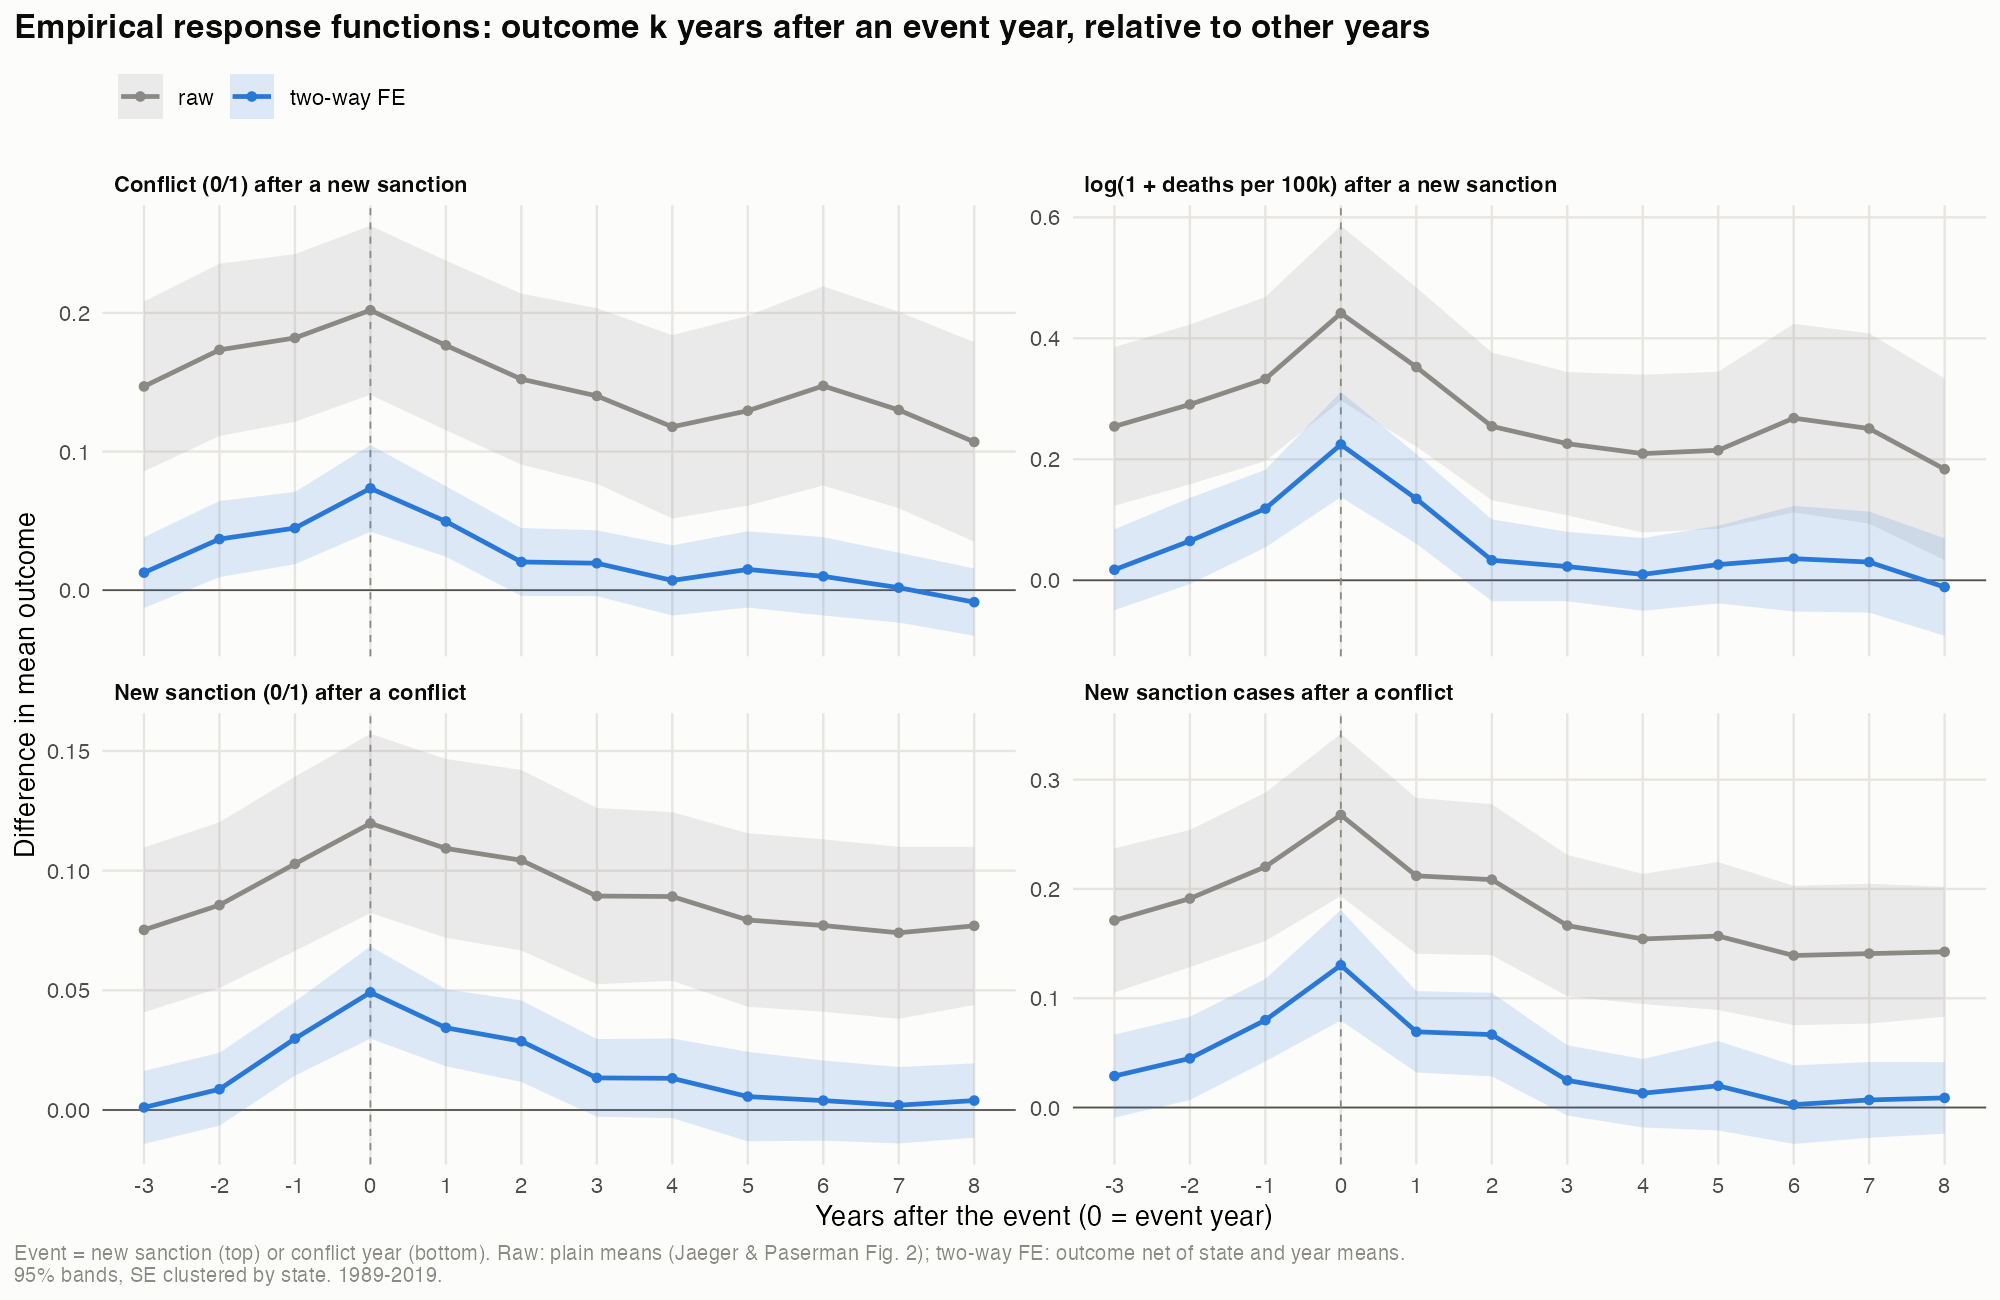
\includegraphics[width=\textwidth]{fig10_response_functions.png}
\caption{Empirical response functions (panel version of \citealt[Fig.~2]{jaeger2008})}
\label{fig:response}
\end{figure}

\subsection{Impulse responses}

Table~\ref{tab:irf} and Figures~\ref{fig:irf}--\ref{fig:cumirf} report the dynamic responses.
\begin{itemize}[leftmargin=*]
\item \textit{Violence shock.} New sanctions respond in 11 of 12 versions. Allowing violence to trigger sanctions
  within the same year roughly doubles the response, so much of the sender reaction is fast.
\item \textit{Sanction shock.} Without a same-year effect, the cumulative response of violence is negative in
  three of four versions and significant for incidence with controls ($-0.077$ conflict-years over ten years) --- a version that relies on
  the sanction-stock control (Section~\ref{sec:controls}).
  If sanctions may affect violence within the year, the response turns positive and significant, because
  sanctions and violence spike in the same year.
\end{itemize}
All VARs are stable; the jackknife responses (dashed in Figure~\ref{fig:irf}) decay more slowly, as expected
once the downward Nickell bias in persistence is removed.

\begin{table}[htbp]
\centering
\footnotesize
\caption{Cumulative impulse responses after ten years}
\label{tab:irf}
\begin{threeparttable}
\begin{tabular}{llccc}
\toprule
 & & \makecell{No same-year\\effect} & \makecell{Cholesky,\\sanctions first} & \makecell{Cholesky,\\violence first} \\
\midrule
\multicolumn{5}{l}{\textit{Shock: new sanction; response: violence}} \\
\quad Incidence & with controls & \makecell{$-$0.077$^{\ast}$\\{\scriptsize[$-$0.154, $-$0.006]}} & \makecell{0.031\\{\scriptsize[$-$0.072, 0.124]}} & \makecell{$-$0.077$^{\ast}$\\{\scriptsize[$-$0.154, $-$0.006]}} \\
\quad Incidence & FE only & \makecell{0.004\\{\scriptsize[$-$0.069, 0.083]}} & \makecell{0.118$^{\ast}$\\{\scriptsize[0.016, 0.223]}} & \makecell{0.004\\{\scriptsize[$-$0.069, 0.083]}} \\
\quad Levels & with controls & \makecell{$-$0.150\\{\scriptsize[$-$0.300, 0.006]}} & \makecell{0.177$^{\ast}$\\{\scriptsize[0.023, 0.355]}} & \makecell{$-$0.150\\{\scriptsize[$-$0.300, 0.006]}} \\
\quad Levels & FE only & \makecell{$-$0.107\\{\scriptsize[$-$0.256, 0.061]}} & \makecell{0.239$^{\ast}$\\{\scriptsize[0.061, 0.477]}} & \makecell{$-$0.107\\{\scriptsize[$-$0.256, 0.061]}} \\
\midrule
\multicolumn{5}{l}{\textit{Shock: violence; response: new sanctions}} \\
\quad Incidence & with controls & \makecell{0.120$^{\ast}$\\{\scriptsize[0.038, 0.210]}} & \makecell{0.120$^{\ast}$\\{\scriptsize[0.038, 0.210]}} & \makecell{0.214$^{\ast}$\\{\scriptsize[0.106, 0.306]}} \\
\quad Incidence & FE only & \makecell{0.159$^{\ast}$\\{\scriptsize[0.066, 0.260]}} & \makecell{0.159$^{\ast}$\\{\scriptsize[0.066, 0.260]}} & \makecell{0.257$^{\ast}$\\{\scriptsize[0.145, 0.369]}} \\
\quad Levels & with controls & \makecell{0.091\\{\scriptsize[$-$0.016, 0.217]}} & \makecell{0.091\\{\scriptsize[$-$0.016, 0.217]}} & \makecell{0.339$^{\ast}$\\{\scriptsize[0.189, 0.495]}} \\
\quad Levels & FE only & \makecell{0.137$^{\ast}$\\{\scriptsize[0.021, 0.260]}} & \makecell{0.137$^{\ast}$\\{\scriptsize[0.021, 0.260]}} & \makecell{0.385$^{\ast}$\\{\scriptsize[0.240, 0.541]}} \\
\bottomrule
\end{tabular}
\begin{tablenotes}[flushleft]\footnotesize
\item \textit{Notes:} Sum of the responses over years 0--10 to a one-unit shock (one new sanction / one conflict year in the incidence VAR; one new case / one unit of $\log(1+$deaths per 100,000$)$ in the levels VAR). 95\% country-cluster bootstrap intervals in brackets (199 draws); $^{\ast}$ interval excludes zero. No same-year effect: the identification of \citet[fn.~12]{jaeger2008}; Cholesky orderings allow a same-year effect in one direction (rescaled to a unit own shock). For a sanction shock, ``no same-year effect'' coincides with ``violence first''; for a violence shock, with ``sanctions first''.
\end{tablenotes}
\end{threeparttable}
\end{table}


\begin{figure}[htbp]
\centering
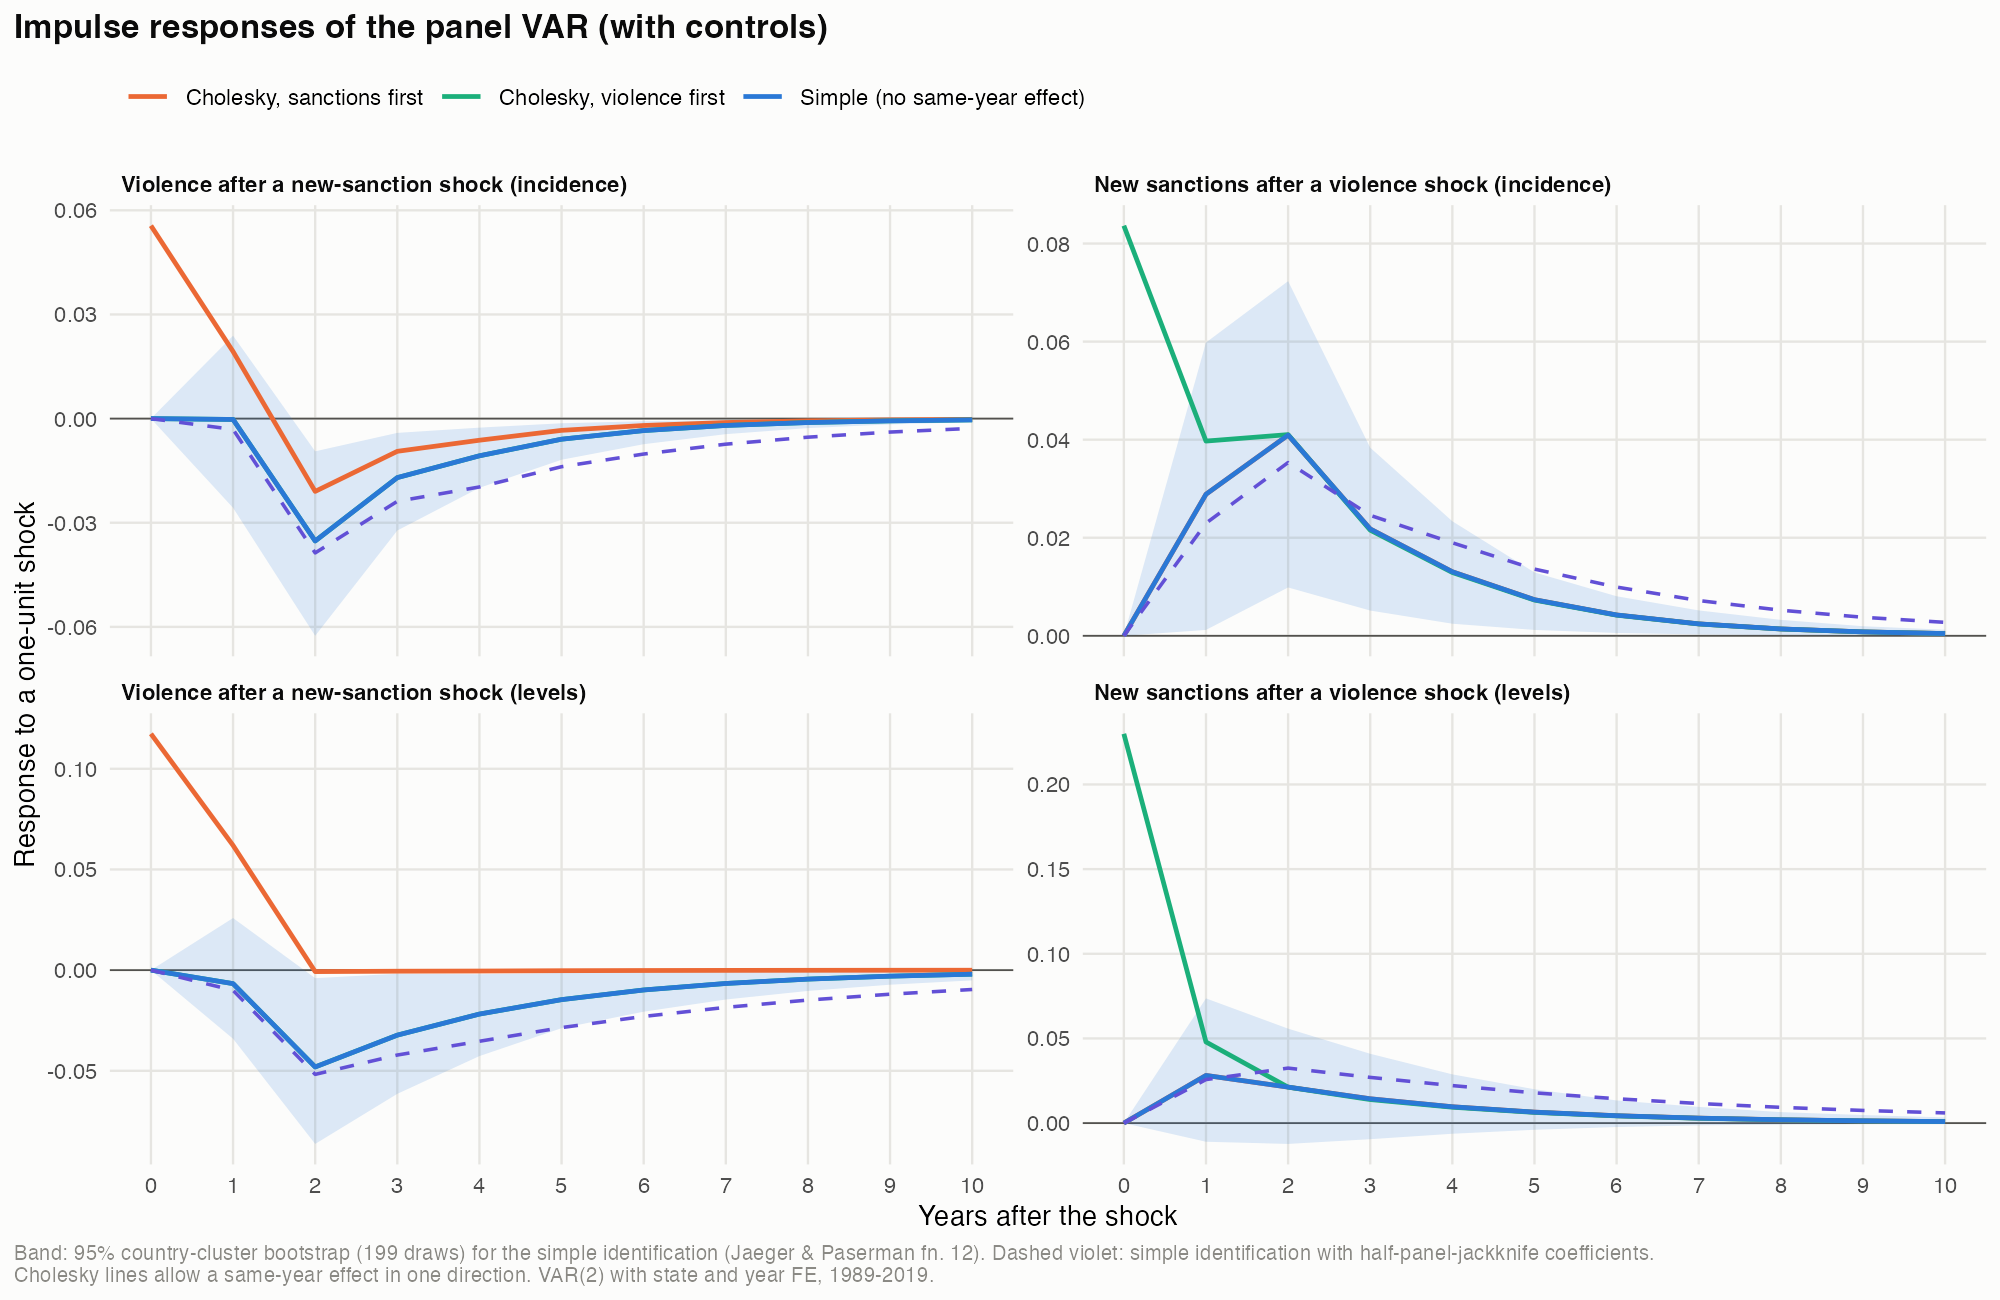
\includegraphics[width=\textwidth]{fig12_irf_with_controls.png}
\caption{Impulse responses, VAR with controls}
\label{fig:irf}
\end{figure}

\begin{figure}[htbp]
\centering
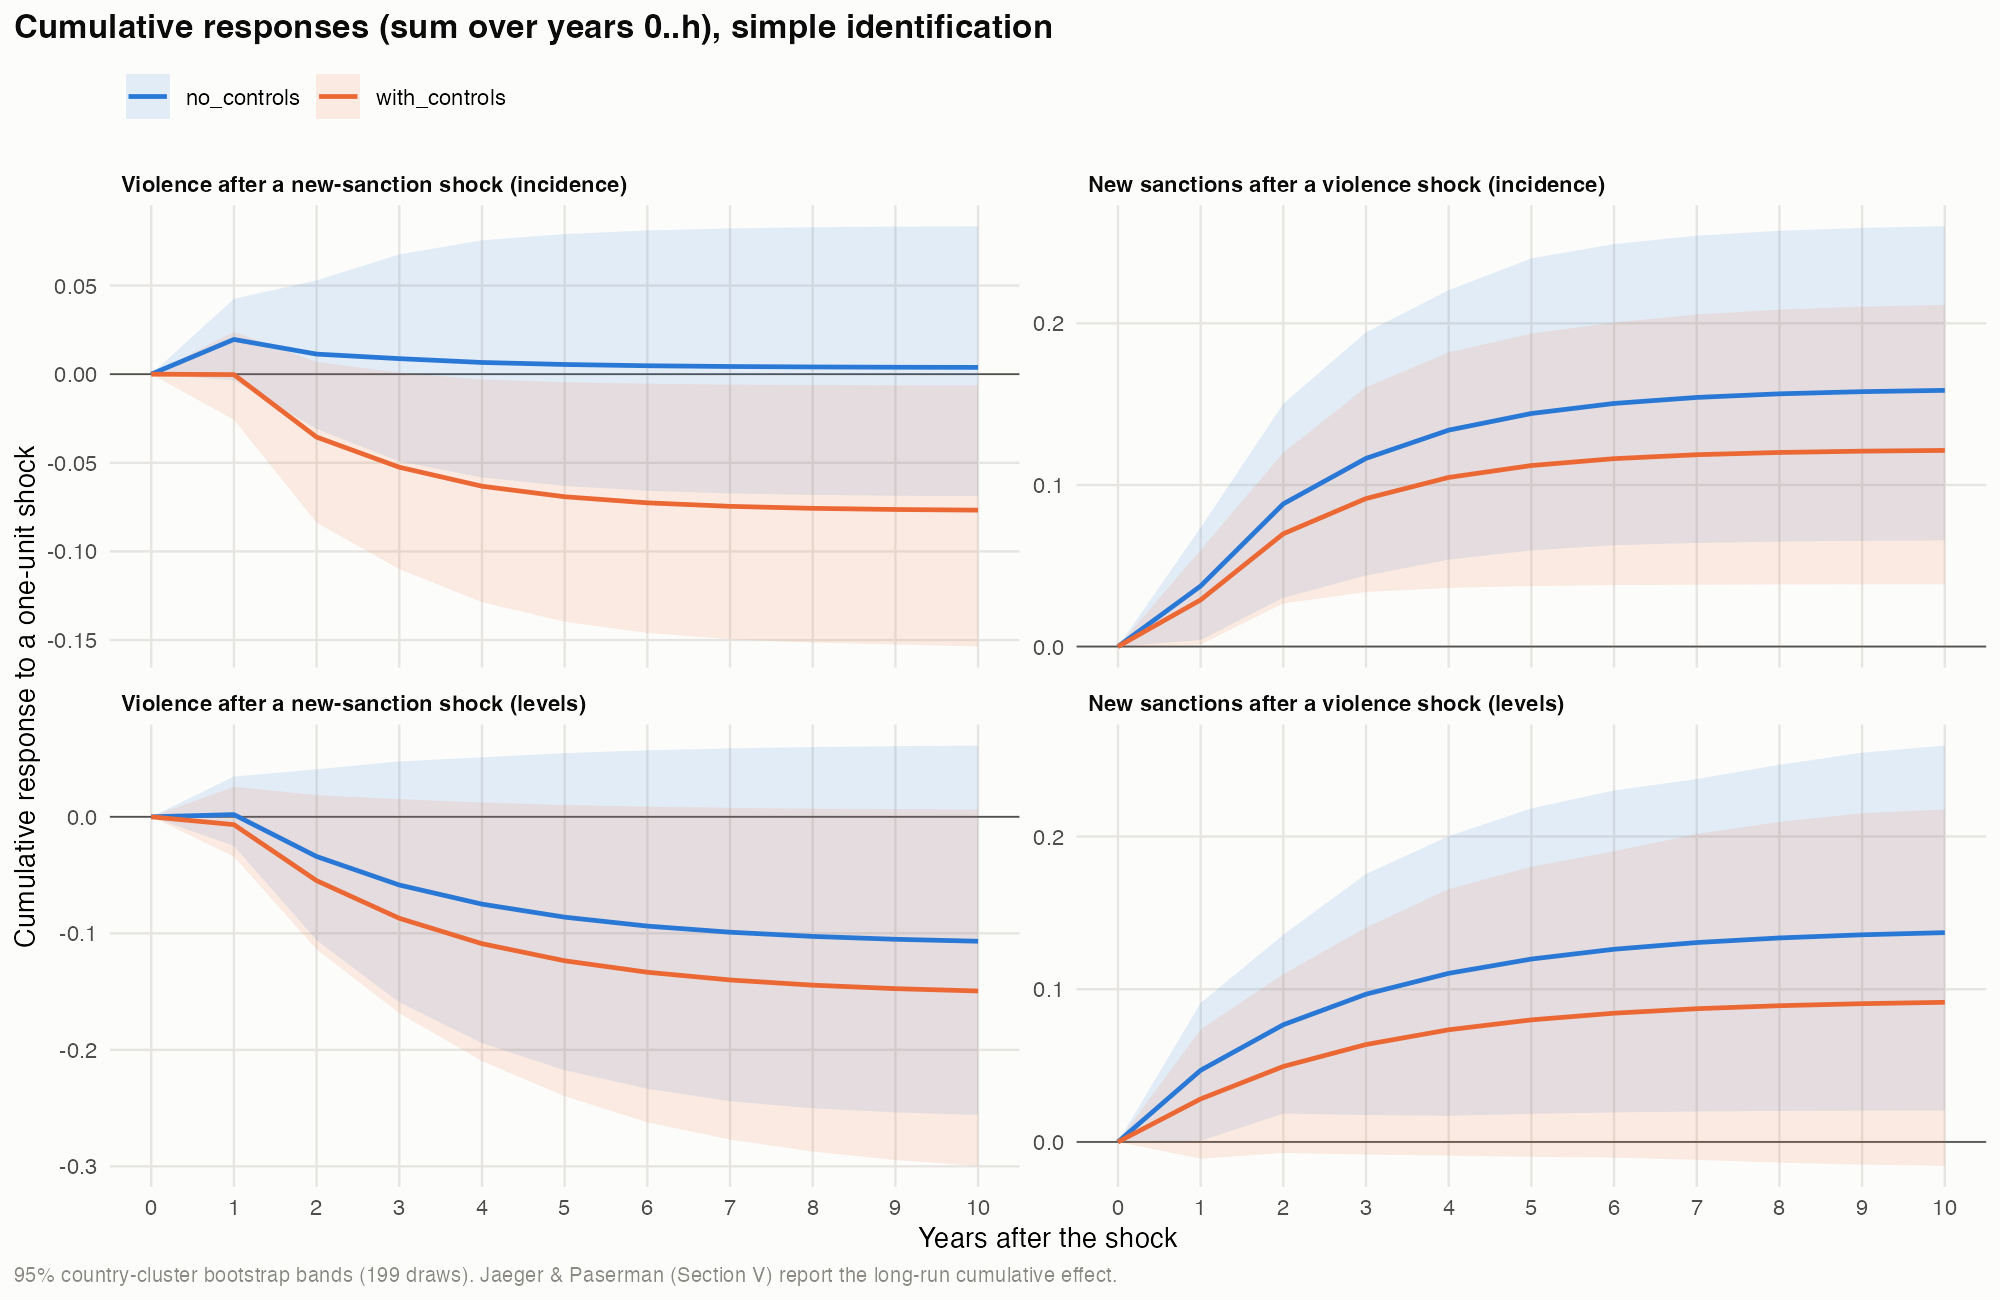
\includegraphics[width=\textwidth]{fig13_cumulative_irf.png}
\caption{Cumulative impulse responses (no same-year effect)}
\label{fig:cumirf}
\end{figure}

% =============================================================================
\section{Diagnostics}
\label{sec:diagnostics}

\paragraph{Stationarity and persistence} (Table~\ref{tab:datadiag}). All four series reject a unit root in the
panel tests, including CIPS, which allows for common shocks. Only states whose series varies can be tested;
constant series (100 states never in conflict) are trivially stationary and stay in the sample. Conflict is
persistent (82\% probability of continuing), new sanctions are close to events. The VAR is therefore estimated
in levels.

\paragraph{Estimated models} (Table~\ref{tab:modeldiag}). The violence equation has no remaining residual
autocorrelation; the sender equation shows a very small one at lag 2 ($p\approx 0.04$), which a third own lag
does not change in substance (Table~\ref{tab:laggrid}). Residuals are weakly correlated across states (mean
correlation 0.01--0.03), consistent with senders acting in waves; Driscoll--Kraay standard errors
\citep{driscoll1998} are planned as a check. All estimated VARs are stable (largest roots 0.56--0.80).

\begin{table}[htbp]
\centering
\footnotesize
\caption{Stationarity and persistence of the VAR variables}
\label{tab:datadiag}
\begin{threeparttable}
\begin{tabular}{lccccccc}
\toprule
 & \multicolumn{4}{c}{Unit-root tests} & \multicolumn{3}{c}{Persistence} \\
\cmidrule(lr){2-5}\cmidrule(lr){6-8}
Series & \makecell{States\\tested} & \makecell{Share\\rejecting} & \makecell{Maddala--Wu,\\Choi $p$} & \makecell{CIPS\\(states)} & \makecell{FE AR(1),\\corrected} & \makecell{P(1$|$0)} & \makecell{P(1$|$1)} \\
\midrule
New sanction (0/1) & 102 & 0.93 & $<$0.001 & $-$3.11 (84) & 0.18 & 0.086 & 0.295 \\
New sanction cases & 102 & 0.92 & $<$0.001 & $-$3.30 (84) & 0.12 &  &  \\
Conflict (0/1) & 62 & 0.53 & $<$0.001 & $-$2.68 (52) & 0.49 & 0.045 & 0.817 \\
log deaths per 100k & 97 & 0.61 & $<$0.001 & $-$3.02 (84) & 0.70 &  &  \\
\bottomrule
\end{tabular}
\begin{tablenotes}[flushleft]\footnotesize
\item \textit{Notes:} Unit-root tests, H$_0$: unit root in every state. State ADF regressions with intercept, 0--2 lagged differences by AIC; Maddala--Wu and Choi combine the state $p$-values (larger of the two shown); CIPS \citep{pesaran2007} adds cross-section averages against common shocks, balanced sub-panel, all $p<0.01$. Only states whose series varies can be tested (constant series, e.g.\ never in conflict, are trivially stationary and stay in the sample). Persistence: FE AR(1) with state and year effects plus the Nickell correction $(1+\rho)/(T-1)$; P(1$|$0), P(1$|$1): probability of a 1 given last year's value. 1989--2019.
\end{tablenotes}
\end{threeparttable}
\end{table}

\begin{table}[htbp]
\centering
\footnotesize
\caption{Diagnostics of the estimated VARs}
\label{tab:modeldiag}
\begin{threeparttable}
\begin{tabular}{llccccccc}
\toprule
 & & \multicolumn{2}{c}{Residual autocorr., $p$} & \multicolumn{2}{c}{Pesaran CD} & \multicolumn{3}{c}{Largest root} \\
\cmidrule(lr){3-4}\cmidrule(lr){5-6}\cmidrule(lr){7-9}
Model & Equation & Lag 1 & Lag 2 & \makecell{Mean\\corr.} & $p$ & OLS & JK & GMM \\
\midrule
Incidence, with controls & Violence & 0.503 & 0.688 & $-$0.007 & 0.023 & 0.57 & 0.72 & 0.56 \\
 & Sender & 0.077 & 0.042 & 0.010 & $<$0.001 &  & &  \\
Incidence, FE only & Violence & 0.566 & 0.804 & $-$0.005 & 0.089 & 0.60 & 0.75 & 0.57 \\
 & Sender & 0.075 & 0.042 & 0.020 & $<$0.001 &  & &  \\
Levels, with controls & Violence & 0.428 & 0.769 & 0.018 & $<$0.001 & 0.67 & 0.80 & 0.67 \\
 & Sender & 0.112 & 0.046 & 0.020 & $<$0.001 &  & &  \\
Levels, FE only & Violence & 0.532 & 0.725 & 0.017 & $<$0.001 & 0.69 & 0.80 & 0.69 \\
 & Sender & 0.094 & 0.044 & 0.029 & $<$0.001 &  & &  \\
\bottomrule
\end{tabular}
\begin{tablenotes}[flushleft]\footnotesize
\item \textit{Notes:} Residual autocorrelation: regression of the FE residual on its own lag, tested against the value $-1/(T-1)$ implied by within-demeaning \citep[section 10.5.4]{wooldridge2010}. Pesaran CD \citep{pesaran2015}: states whose dependent variable varies (constant-outcome states have mechanically identical residuals); mean pairwise residual correlation and $p$-value. Largest root: modulus of the largest eigenvalue of the companion matrix (stable if $<1$), FE-OLS, half-panel jackknife (JK) and GMM.
\end{tablenotes}
\end{threeparttable}
\end{table}


% =============================================================================
\section{Robustness}
\label{sec:robustness}

\subsection{GMM}
GMM removes the Nickell bias by construction. It confirms the sanctions$\rightarrow$violence results in all four
versions (Table~\ref{tab:granger}) and the levels results for violence$\rightarrow$sanctions. The Hansen test
does not reject in the levels models; it rejects for incidence without controls, so the GMM incidence results are
the least reliable (Table~\ref{tab:gmm}).

\begin{table}[htbp]
\centering
\small
\caption{GMM panel VAR: specification tests}
\label{tab:gmm}
\begin{threeparttable}
\begin{tabular}{lcccccc}
\toprule
Specification & States & Obs. & Moments & Hansen $J$ (df) & $p$ & Largest root \\
\midrule
Incidence, with controls & 174 & 4,739 & 24 & 14.56 (8) & 0.068 & 0.56 \\
Incidence, FE only & 197 & 5,341 & 16 & 16.50 (8) & 0.036 & 0.57 \\
Levels, with controls & 174 & 4,739 & 24 & 8.32 (8) & 0.403 & 0.67 \\
Levels, FE only & 197 & 5,341 & 16 & 7.60 (8) & 0.473 & 0.69 \\
\bottomrule
\end{tabular}
\begin{tablenotes}[flushleft]\footnotesize
\item \textit{Notes:} Two-step GMM with forward orthogonal deviations and collapsed instruments (lags 2--5), variables demeaned by year \citep{abrigo2016}. Hansen $J$: H$_0$ instruments valid \citep{hansen1982}; the number of moment conditions stays well below the number of states \citep{roodman2009}.
\end{tablenotes}
\end{threeparttable}
\end{table}


\subsection{Nonlinear models: logit and PPML}
% NUMBERS: Table tab:nonlinear (run 2026-10-23 16:50)

\paragraph{Why.} The base-case reaction functions are linear: linear probability models for incidence and OLS on
$\log(1+\text{deaths per }100{,}000)$ for levels. Both choices are convenient but questionable with outcomes that
are zero in most state-years. A linear probability model can predict outside $[0,1]$ and imposes a constant
marginal effect regardless of how likely conflict already is. A $\log(1+y)$ outcome has no percentage
interpretation when many observations are zero, and its coefficients change with the units in which $y$ is
measured \citep{chen2024}. \citet[fn.~3]{jaeger2008} address the same concern in their data with probit and
zero-inflated Poisson regressions.

\paragraph{Design.} We re-estimate every reaction function of Table~\ref{tab:granger} with a model suited to its
outcome, keeping the samples, the two lags, the controls, the state and year fixed effects and the clustering by
state unchanged (Table~\ref{tab:nonlinear}):
\begin{itemize}[leftmargin=*]
\item \emph{Logit} for the incidence equations (conflict 0/1, new sanction 0/1). To compare magnitudes with the
  linear model, the sum of the lag coefficients is converted into an approximate average partial effect on the
  probability.
\item \emph{Poisson pseudo-maximum likelihood} \citep[PPML;][]{santossilva2006} for the levels equations, with the
  \emph{untransformed} outcome: deaths per 100,000 and the number of new cases. PPML is consistent for any
  non-negative outcome with an exponential mean, handles zeros naturally and gives coefficients that are
  semi-elasticities. Because the death rate is extremely skewed (Rwanda 1994 alone has 12,577 deaths per
  100,000), we also report a version with deaths winsorised at the 99th percentile (45.6).
\end{itemize}
With fixed effects, states whose outcome never changes carry no information and drop out: in the conflict logit
85--108 states with an unchanged conflict status (mostly states never in conflict), in the deaths PPML 61--84
states without any deaths, in the sender models 19--32 states never newly sanctioned.

\paragraph{Sanctions $\rightarrow$ violence.} The pattern of the linear models holds in every version: the
coefficient on the first lag of new sanctions is close to zero, the coefficient on the second lag is negative.
\begin{itemize}[leftmargin=*]
\item \emph{Logit, with controls:} the lags are jointly significant ($p=0.040$); the average partial effect of
  $-0.046$ is close to the linear-probability estimate of $-0.035$, i.e.\ about a 4--5 percentage-point lower
  probability of conflict two years after a new sanction (mean 0.23). \emph{Without controls,} the first lag turns
  positive and offsets the second ($p=0.058$, average partial effect $\approx 0$), exactly as in the linear model.
  As there, the incidence result with controls depends on the sanction-stock control (Section~\ref{sec:controls}).
\item \emph{PPML on raw deaths:} the point estimates are large --- death rates about a quarter to a third lower
  two years after a sanction --- but imprecise ($p=0.14$ with controls, $0.25$ without). A Poisson likelihood
  weights observations by their size, so a handful of extreme state-years determine the estimate.
\item \emph{PPML on winsorised deaths:} once the extreme values are capped, the effect is precisely estimated
  ($p=0.002$ with and without controls): death rates are 11--16\% lower two years after a new sanction.
\end{itemize}

\paragraph{Violence $\rightarrow$ sanctions.} Also unchanged. Without controls, past violence predicts new
sanctions in the logit ($p=0.006$; a conflict year raises the probability of a new sanction by about 6 percentage
points over the next two years) and in the PPML ($p=0.024$; 15\% more new cases per unit of log deaths). With
controls both weaken (logit $p=0.065$, PPML $p=0.46$), the same pattern as in the linear model, where GDP growth
absorbs part of the sender reaction.

\paragraph{What the check adds and what it does not.} The linear specification is not what drives the results:
signs, lag pattern and significance survive a change of functional form, and the logit magnitudes are close to
the linear ones. The PPML results also show that the levels finding does not depend on the $\log(1+y)$
transformation; on the contrary, the semi-elasticities give the effect a natural scale (an 11--16\% lower death
rate). Three caveats remain.
\begin{enumerate}[leftmargin=*]
\item \emph{Different identifying sample.} Because states without variation drop out, the nonlinear models
  identify the effect from states that experience conflict at some point. The agreement with the linear models,
  which use all states, suggests that the never-violent states do not drive the linear estimates either; this is
  related to the conflict-prone subsample (decision D7).
\item \emph{Incidental-parameter bias.} Fixed-effects logit with $T\approx 29$ has a bias of order $1/T$, the
  nonlinear counterpart of the Nickell bias; an analytical correction is a possible refinement. PPML with fixed
  effects does not have this problem for exogenous regressors, but the lagged outcome makes the regressors only
  predetermined.
\item \emph{Sensitivity to extreme values.} The comparison of raw and winsorised PPML shows that the effect comes
  from the bulk of conflict state-years; the largest atrocities add noise rather than drive it. The cap at the
  99th percentile is a choice, and other caps (95th, 99.5th) would be a natural check.
\end{enumerate}
The functional-form check therefore strengthens the base-case reading: the small reduction in violence two years
after a sanction, conditional on the controls, is not an artefact of linear models or of the log transformation;
the same-year timing problem (Section~\ref{sec:results}) is unaffected by it.

\begin{table}[htbp]
\centering
\scriptsize\setlength{\tabcolsep}{3pt}
\caption{Robustness: logit and PPML versions of the reaction functions}
\label{tab:nonlinear}
\begin{threeparttable}
\begin{tabular}{llccccccc}
\toprule
 & & \multicolumn{2}{c}{Linear (Table~\ref{tab:granger})} & \multicolumn{4}{c}{Nonlinear} & \\
\cmidrule(lr){3-4}\cmidrule(lr){5-8}
Model & Controls & $\chi^2(2)$ & Sum & $\chi^2(2)$ & Lag $t-1$ & Lag $t-2$ & \makecell{Sum, comparable\\scale} & \makecell{States\\(dropped)} \\
\midrule
\multicolumn{9}{l}{\textit{Sanctions $\rightarrow$ violence}} \\
\quad Logit & with controls & 7.27$^{**}$ & $-$0.035 & 6.44$^{**}$ & 0.022 & $-$0.476 & APE $-$0.046 & 89 (85) \\
\quad Logit & FE only & 5.01$^{*}$ & 0.002 & 5.69$^{*}$ & 0.322 & $-$0.259 & APE 0.007 & 89 (108) \\
\quad PPML & with controls & 8.08$^{**}$ & $-$0.050 & 3.94 & $-$0.008 & $-$0.401 & $-$0.410 ($-$34\%) & 113 (61) \\
\quad PPML & FE only & 7.14$^{**}$ & $-$0.035 & 2.75 & 0.091 & $-$0.383 & $-$0.291 ($-$25\%) & 113 (84) \\
\quad PPML, winsorised & with controls & 8.08$^{**}$ & $-$0.050 & 12.52$^{***}$ & $-$0.004 & $-$0.166 & $-$0.171 ($-$16\%) & 113 (61) \\
\quad PPML, winsorised & FE only & 7.14$^{**}$ & $-$0.035 & 11.99$^{***}$ & 0.023 & $-$0.141 & $-$0.117 ($-$11\%) & 113 (84) \\
\midrule
\multicolumn{9}{l}{\textit{Violence $\rightarrow$ sanctions}} \\
\quad Logit & with controls & 6.11$^{**}$ & 0.055 & 5.48$^{*}$ & 0.293 & 0.221 & APE 0.046 & 155 (19) \\
\quad Logit & FE only & 9.86$^{***}$ & 0.070 & 10.21$^{***}$ & 0.402 & 0.273 & APE 0.058 & 165 (32) \\
\quad PPML & with controls & 2.79 & 0.030 & 1.54 & 0.011 & 0.060 & 0.071 (+7\%) & 155 (19) \\
\quad PPML & FE only & 7.30$^{**}$ & 0.045 & 7.43$^{**}$ & 0.127 & 0.011 & 0.137 (+15\%) & 165 (32) \\
\bottomrule
\end{tabular}
\begin{tablenotes}[flushleft]\footnotesize
\item \textit{Notes:} Same samples, two lags, controls, state and year fixed effects and clustering as Table~\ref{tab:granger}; fixed effects as dummies. Logit: incidence equations (conflict 0/1, new sanction 0/1); APE = sum of the two lag coefficients $\times$ mean $\hat p(1-\hat p)$, an approximate average partial effect comparable to the linear-probability sum. PPML \citep{santossilva2006}: levels equations with untransformed outcomes (deaths per 100,000, also winsorised at the 99th percentile; number of new cases), right-hand side as in the levels VAR; sum in log points and implied proportional change. States whose outcome never varies carry no information with fixed effects and are dropped. $^{*}p<0.1$, $^{**}p<0.05$, $^{***}p<0.01$.
\end{tablenotes}
\end{threeparttable}
\end{table}


\subsection{Raw instead of log deaths}
% NUMBERS: Table tab:rawdeaths (run 2026-10-23 16:50)
\citet{jaeger2008} estimate their levels VAR on raw fatality counts. Our base case uses
$\log(1+\text{deaths per }100{,}000)$ because the death rate is extremely skewed. Table~\ref{tab:rawdeaths}
re-estimates the linear levels VAR with deaths per 100,000 instead, uncapped and winsorised at the 99th (45.6)
and 95th (6.2) percentile of all state-years; the cap applies to the outcome and to its lags. Everything else is
as in Table~\ref{tab:granger}.
\begin{itemize}[leftmargin=*]
\item \textit{Uncapped raw deaths are not informative.} A single observation dominates the estimates: Rwanda's
  12,577 deaths per 100,000 in 1994. It pulls the estimated persistence of violence down to 0.17 (0.67 with log
  deaths), and in the sender equation it produces an absurd Granger statistic ($\chi^2\approx 300$), because
  Rwanda received two new sanction cases in 1996; without Rwanda the statistic falls to 4.7 ($p=0.10$). This is
  the reason for the transformation in the base case.
\item \textit{Capped deaths: sanctions $\rightarrow$ violence holds.} With either cap, the lags of new sanctions are
  jointly significant with controls ($p=0.036$ at p99, $p=0.025$ at p95) and marginally without ($p\approx
  0.055$), with negative sums: about 0.34 (p99) and 0.10 (p95) fewer deaths per 100,000 two years after a new
  case, i.e.\ roughly 17--24\% of the mean of the capped variable.
\item \textit{Violence $\rightarrow$ sanctions} is significant without controls at the p99 cap ($p=0.001$) and
  weaker with controls or with the stronger p95 cap, the same pattern as in the base case.
\end{itemize}
The base-case results therefore do not depend on the log transformation as long as the most extreme
state-years are capped; the uncapped raw-count version, the analogue of \citet{jaeger2008}, is unsuitable for a
cross-country panel that includes a genocide.

\begin{table}[htbp]
\centering
\footnotesize
\caption{Robustness: raw instead of log deaths in the levels VAR}
\label{tab:rawdeaths}
\begin{threeparttable}
\begin{tabular}{lcccc}
\toprule
 & \makecell{log(1+deaths)\\(Table~\ref{tab:granger})} & \makecell{Raw\\deaths} & \makecell{Capped at p99\\(45.6)} & \makecell{Capped at p95\\(6.2)} \\
\midrule
\multicolumn{5}{l}{\textit{Sanctions $\rightarrow$ violence}} \\
\quad with controls & \makecell{8.08$^{**}$\\{\scriptsize [$-$0.050]}} & \makecell{0.55\\{\scriptsize [$-$2.534]}} & \makecell{6.63$^{**}$\\{\scriptsize [$-$0.338]}} & \makecell{7.41$^{**}$\\{\scriptsize [$-$0.096]}} \\
\quad FE only & \makecell{7.14$^{**}$\\{\scriptsize [$-$0.035]}} & \makecell{4.18\\{\scriptsize [0.563]}} & \makecell{5.68$^{*}$\\{\scriptsize [$-$0.186]}} & \makecell{5.82$^{*}$\\{\scriptsize [$-$0.067]}} \\
\midrule
\multicolumn{5}{l}{\textit{Violence $\rightarrow$ sanctions}} \\
\quad with controls & \makecell{2.79\\{\scriptsize [0.030]}} & \makecell{289.58$^{***}$\\{\scriptsize [0.0001]}} & \makecell{4.55\\{\scriptsize [0.0029]}} & \makecell{1.99\\{\scriptsize [0.0168]}} \\
\quad FE only & \makecell{7.30$^{**}$\\{\scriptsize [0.045]}} & \makecell{323.10$^{***}$\\{\scriptsize [0.0001]}} & \makecell{13.94$^{***}$\\{\scriptsize [0.0048]}} & \makecell{4.32\\{\scriptsize [0.0236]}} \\
\midrule
Largest root (OLS) & 0.67--0.69 & 0.17--0.18 & 0.57--0.58 & 0.69--0.70 \\
Mean of violence variable & 0.29 & 5.02 & 1.42 & 0.56 \\
\bottomrule
\end{tabular}
\begin{tablenotes}[flushleft]\footnotesize
\item \textit{Notes:} FE-OLS levels VAR(2) as in Table~\ref{tab:granger}, with deaths per 100,000 instead of $\log(1+$deaths per 100,000$)$ as the violence variable (outcome and lags), as in the raw-count specification of \citet{jaeger2008}. Caps at the 99th and 95th percentile of all state-years 1989--2019 (deaths per 100,000 in parentheses). Granger $\chi^2(2)$; sum of the two cross-lag coefficients in brackets (sanctions$\rightarrow$violence: deaths per 100,000 per new case; violence$\rightarrow$sanctions: new cases per death per 100,000). Jackknife versions in \texttt{robustness\_raw\_deaths.csv}. $^{*}p<0.1$, $^{**}p<0.05$, $^{***}p<0.01$.
\end{tablenotes}
\end{threeparttable}
\end{table}


\paragraph{Dynamics in deaths rather than log points.} Because the capped version is still a linear VAR, it also
delivers impulse responses in an interpretable unit, deaths per 100,000 --- the analogue of the long-run numbers
in \citet[Section V]{jaeger2008}. Table~\ref{tab:cappedirf} and Figure~\ref{fig:capped} use the p99 cap.
\begin{itemize}[leftmargin=*]
\item \textit{New sanction $\rightarrow$ deaths.} Without a same-year effect, one new sanction case is followed by
  0.8 fewer deaths per 100,000 over ten years with controls (0.5 without), about half a year's average death rate
  (1.42). The sign matches the log version, but the bootstrap intervals include zero: with deaths in levels, the
  dynamics are estimated less precisely than the Granger test. If sanctions may affect deaths within the same year,
  the cumulative response is positive (+1.1 to +1.6), as in the base case.
\item \textit{Deaths $\rightarrow$ new sanctions.} One additional death per 100,000 raises the number of new cases
  by about 0.01 over ten years (significant without controls), and by 0.03--0.04 if deaths may trigger sanctions
  within the same year (significant in all versions). Senders react, but per death the reaction is small.
\item \textit{Response function.} Capped deaths are already above normal in the year before a new sanction,
  peak in the sanction year (+1.8 deaths per 100,000 relative to the state's normal level) and are back to normal
  two years later --- the same shape as with log deaths (Figure~\ref{fig:response}).
\end{itemize}

\begin{table}[htbp]
\centering
\footnotesize
\caption{Cumulative impulse responses after ten years, levels VAR with capped deaths}
\label{tab:cappedirf}
\begin{threeparttable}
\begin{tabular}{lccc}
\toprule
 & \makecell{No same-year\\effect} & \makecell{Cholesky,\\sanctions first} & \makecell{Cholesky,\\violence first} \\
\midrule
\multicolumn{4}{l}{\textit{One new sanction case $\rightarrow$ deaths per 100,000}} \\
\quad with controls & \makecell{$-$0.827\\{\scriptsize[$-$1.985, 0.206]}} & \makecell{1.079$^{\ast}$\\{\scriptsize[0.032, 2.330]}} & \makecell{$-$0.827\\{\scriptsize[$-$1.985, 0.206]}} \\
\quad FE only & \makecell{$-$0.465\\{\scriptsize[$-$1.587, 0.609]}} & \makecell{1.600$^{\ast}$\\{\scriptsize[0.358, 3.241]}} & \makecell{$-$0.465\\{\scriptsize[$-$1.587, 0.609]}} \\
\midrule
\multicolumn{4}{l}{\textit{+1 death per 100,000 $\rightarrow$ new sanction cases}} \\
\quad with controls & \makecell{0.007\\{\scriptsize[$-$0.002, 0.016]}} & \makecell{0.007\\{\scriptsize[$-$0.002, 0.016]}} & \makecell{0.031$^{\ast}$\\{\scriptsize[0.017, 0.047]}} \\
\quad FE only & \makecell{0.012$^{\ast}$\\{\scriptsize[0.003, 0.022]}} & \makecell{0.012$^{\ast}$\\{\scriptsize[0.003, 0.022]}} & \makecell{0.036$^{\ast}$\\{\scriptsize[0.023, 0.053]}} \\
\bottomrule
\end{tabular}
\begin{tablenotes}[flushleft]\footnotesize
\item \textit{Notes:} Levels VAR(2) with deaths per 100,000 capped at the 99th percentile (45.6) instead of log deaths; state and year fixed effects. Sum of the responses over years 0--10 to one new sanction case or to one additional death per 100,000; 95\% country-cluster bootstrap intervals in brackets (199 draws); $^{\ast}$ interval excludes zero. Identifications as in Table~\ref{tab:irf}.
\end{tablenotes}
\end{threeparttable}
\end{table}


\paragraph{Reading Figure~\ref{fig:capped}.} The three panels show the timing behind these numbers.
% NUMBERS: robustness_capped_irf.csv, robustness_capped_response.csv (run 2026-10-23 16:50)
\begin{itemize}[leftmargin=*]
\item \textit{Left panel (deaths after a new case).} Nothing happens in the year after the sanction (cumulative
  response $-0.01$ with controls, $+0.08$ without). The decline starts in the second year ($-0.33$ and $-0.21$
  deaths per 100,000 in that year alone), continues more weakly in the third, and has run its course after about
  five years, when the cumulative curve flattens at $-0.8$ (with controls) and $-0.5$ (without). This is the
  $t-2$ pattern of the Granger tests seen as a dynamic path. The bands are wide and include zero at every horizon,
  so the panel shows the direction and timing, not a precisely estimated effect.
\item \textit{Middle panel (new cases after one additional death per 100,000).} The sender reaction comes
  quickly: most of it in the first year after the violence shock (0.005--0.007 new cases), a little more in the
  second, and nothing after year three. Without controls the band excludes zero from the first year on; with
  controls it touches zero.
\item \textit{Right panel (deaths around a new-sanction year).} The grey line (raw means) is above zero at every
  horizon, including three years \emph{before} the sanction: sanctioned states are more violent in general, by
  1--3 deaths per 100,000. Net of state and year means (green), deaths are at their normal level three and two
  years before a sanction, rise in the year before ($+1.0$), peak in the sanction year ($+1.8$), are still elevated
  one year later ($+1.0$) and are back to normal from the second year on, where they stay.
\end{itemize}
Read together, the left and right panels say the same thing as the log version: the decline that the VAR attributes
to sanctions begins exactly when the escalation around the sanction year ends. Whether sanctions shorten that
escalation or merely coincide with its end cannot be decided from annual data. What the figure does not show
is any sign of a lasting \emph{increase} in deaths after sanctions: two years on, deaths are back at the state's
normal level, and in the VAR, which conditions on the sanction-year escalation, the point estimates are negative.

\begin{figure}[htbp]
\centering
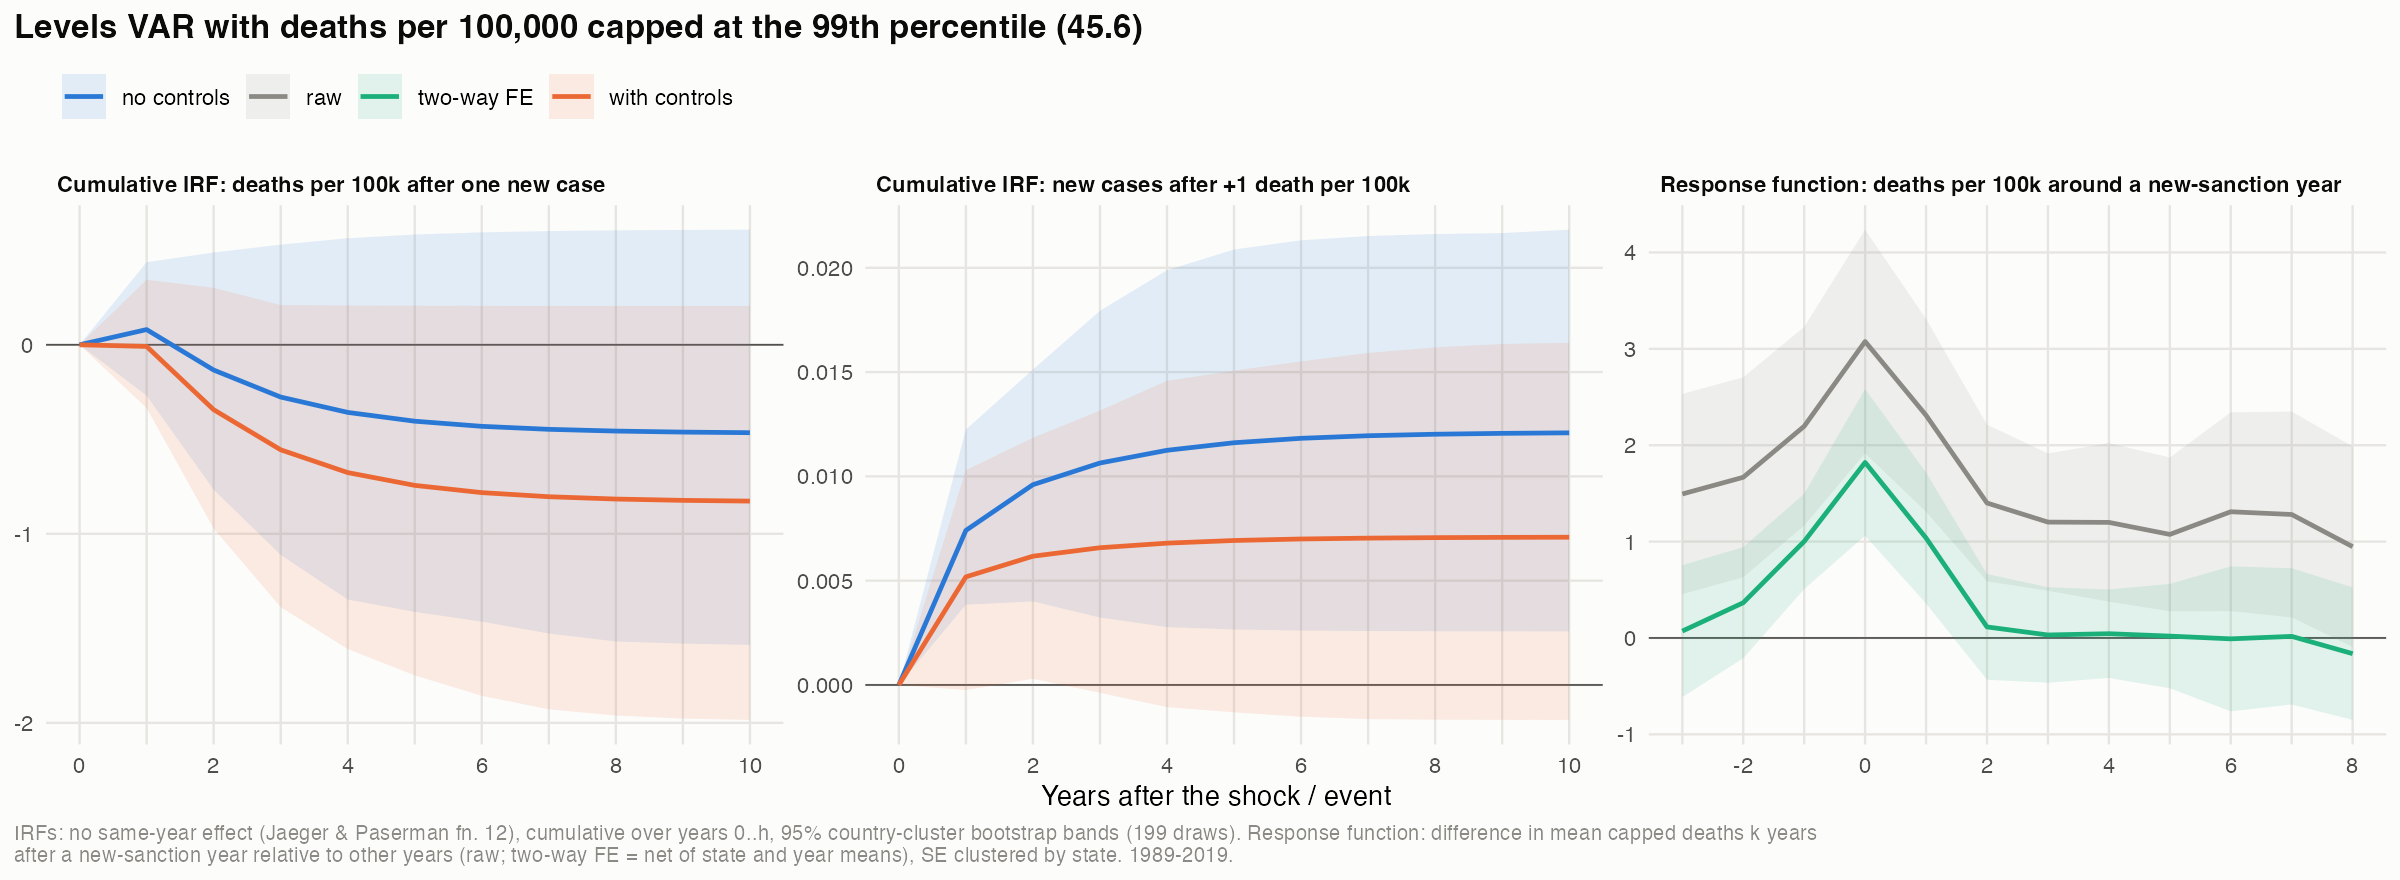
\includegraphics[width=\textwidth]{fig17_capped_deaths_dynamics.png}
\caption{Levels VAR with deaths per 100,000 capped at the 99th percentile: cumulative impulse responses and
response function}
\label{fig:capped}
\end{figure}

\subsection{GDELT instead of UCDP}
Table~\ref{tab:gdelt} repeats the Granger tests with media-reported violence.
\begin{itemize}[leftmargin=*]
\item \textit{Sanctions $\rightarrow$ violence.} Incidence with controls: a sum of lag coefficients of $-0.032$, almost
  identical to UCDP ($-0.035$) but not significant. Levels: positive and significant, i.e.\ more reported
  low-level violence after sanctions; the response functions show the violent share up by 0.5--0.7
  percentage points in the sanction year and the year after (Figure~\ref{fig:gdeltresponse}).
\item \textit{Violence $\rightarrow$ sanctions.} Not found with GDELT. The GDELT incidence measure tracks UCDP
  conflict poorly, however (Table~\ref{tab:gdeltvalidation}): a UCDP conflict year is above the state's GDELT
  median only 64\% of the time. This is a weak test rather than a contradiction.
\end{itemize}
One possible reading: sanctions are followed by fewer deaths but more low-level unrest. This
needs a better GDELT incidence definition before it can be claimed.

\begin{table}[htbp]
\centering
\footnotesize
\caption{Robustness: Granger tests with GDELT instead of UCDP violence}
\label{tab:gdelt}
\begin{threeparttable}
\begin{tabular}{llccccc}
\toprule
 & & UCDP & \multicolumn{4}{c}{GDELT} \\
\cmidrule(lr){3-3}\cmidrule(lr){4-7}
 & & \makecell{1991--2019\\OLS} & \makecell{1991--2019\\OLS} & \makecell{1981--2021\\OLS} & \makecell{$\geq$100 events\\OLS} & \makecell{1991--2019\\jackknife} \\
\midrule
\multicolumn{7}{l}{\textit{Sanctions $\rightarrow$ violence}} \\
\quad Incidence & with controls & \makecell{7.27$^{**}$\\{\scriptsize [$-$0.035]}} & \makecell{3.85\\{\scriptsize [$-$0.032]}} & \makecell{2.39\\{\scriptsize [$-$0.015]}} & \makecell{4.21\\{\scriptsize [$-$0.032]}} & \makecell{4.28\\{\scriptsize [$-$0.037]}} \\
\quad Incidence & FE only & \makecell{5.01$^{*}$\\{\scriptsize [0.002]}} & \makecell{4.47\\{\scriptsize [0.010]}} & \makecell{4.21\\{\scriptsize [0.021]}} & \makecell{4.79$^{*}$\\{\scriptsize [0.010]}} & \makecell{5.46$^{*}$\\{\scriptsize [0.023]}} \\
\quad Levels & with controls & \makecell{8.08$^{**}$\\{\scriptsize [$-$0.050]}} & \makecell{7.19$^{**}$\\{\scriptsize [0.027]}} & \makecell{4.19\\{\scriptsize [$-$0.025]}} & \makecell{7.77$^{**}$\\{\scriptsize [0.027]}} & \makecell{8.09$^{**}$\\{\scriptsize [0.039]}} \\
\quad Levels & FE only & \makecell{7.14$^{**}$\\{\scriptsize [$-$0.035]}} & \makecell{11.18$^{***}$\\{\scriptsize [0.143]}} & \makecell{6.08$^{**}$\\{\scriptsize [0.097]}} & \makecell{9.16$^{**}$\\{\scriptsize [0.091]}} & \makecell{13.65$^{***}$\\{\scriptsize [0.216]}} \\
\midrule
\multicolumn{7}{l}{\textit{Violence $\rightarrow$ sanctions}} \\
\quad Incidence & with controls & \makecell{6.11$^{**}$\\{\scriptsize [0.055]}} & \makecell{1.44\\{\scriptsize [$-$0.012]}} & \makecell{0.38\\{\scriptsize [0.005]}} & \makecell{1.20\\{\scriptsize [$-$0.011]}} & \makecell{0.42\\{\scriptsize [$-$0.006]}} \\
\quad Incidence & FE only & \makecell{9.86$^{***}$\\{\scriptsize [0.070]}} & \makecell{0.45\\{\scriptsize [$-$0.006]}} & \makecell{0.67\\{\scriptsize [0.007]}} & \makecell{0.34\\{\scriptsize [$-$0.006]}} & \makecell{0.10\\{\scriptsize [0.002]}} \\
\quad Levels & with controls & \makecell{2.79\\{\scriptsize [0.030]}} & \makecell{1.28\\{\scriptsize [0.004]}} & \makecell{1.80\\{\scriptsize [0.004]}} & \makecell{1.17\\{\scriptsize [0.004]}} & \makecell{6.16$^{**}$\\{\scriptsize [0.010]}} \\
\quad Levels & FE only & \makecell{7.30$^{**}$\\{\scriptsize [0.045]}} & \makecell{2.14\\{\scriptsize [0.005]}} & \makecell{2.59\\{\scriptsize [0.004]}} & \makecell{2.18\\{\scriptsize [0.005]}} & \makecell{12.78$^{***}$\\{\scriptsize [0.013]}} \\
\bottomrule
\end{tabular}
\begin{tablenotes}[flushleft]\footnotesize
\item \textit{Notes:} $\chi^2(2)$ Granger statistic, sum of the two lag coefficients in brackets. GDELT violence: assault, fight and mass-violence events per 100 GDELT events in the state-year \citep{leetaru2013}; incidence = 1 if above the state's own 1979--2021 median. ``$\geq$100 events'': state-years with fewer than 100 GDELT events set to missing. Units differ from UCDP, so compare signs and significance. $^{*}p<0.1$, $^{**}p<0.05$, $^{***}p<0.01$.
\end{tablenotes}
\end{threeparttable}
\end{table}

\begin{table}[htbp]
\centering
\small
\caption{How closely does GDELT track UCDP violence?}
\label{tab:gdeltvalidation}
\begin{threeparttable}
\begin{tabular}{lc}
\toprule
Statistic & Value \\
\midrule
Correlation with UCDP log deaths, pooled & 0.61 \\
Correlation with UCDP log deaths, within states & 0.47 \\
Correlation with UCDP conflict (0/1), pooled & 0.58 \\
Correlation with UCDP conflict (0/1), within states & 0.38 \\
P(GDELT incidence $=1$ $|$ UCDP conflict year) & 0.64 \\
P(GDELT incidence $=1$ $|$ no UCDP conflict) & 0.46 \\
P(UCDP conflict $|$ GDELT incidence $=1$) & 0.27 \\
\bottomrule
\end{tabular}
\begin{tablenotes}[flushleft]\footnotesize
\item \textit{Notes:} State-years 1989--2019 with both measures. GDELT measure: violent events in \% of all GDELT events.
\end{tablenotes}
\end{threeparttable}
\end{table}


\begin{figure}[htbp]
\centering
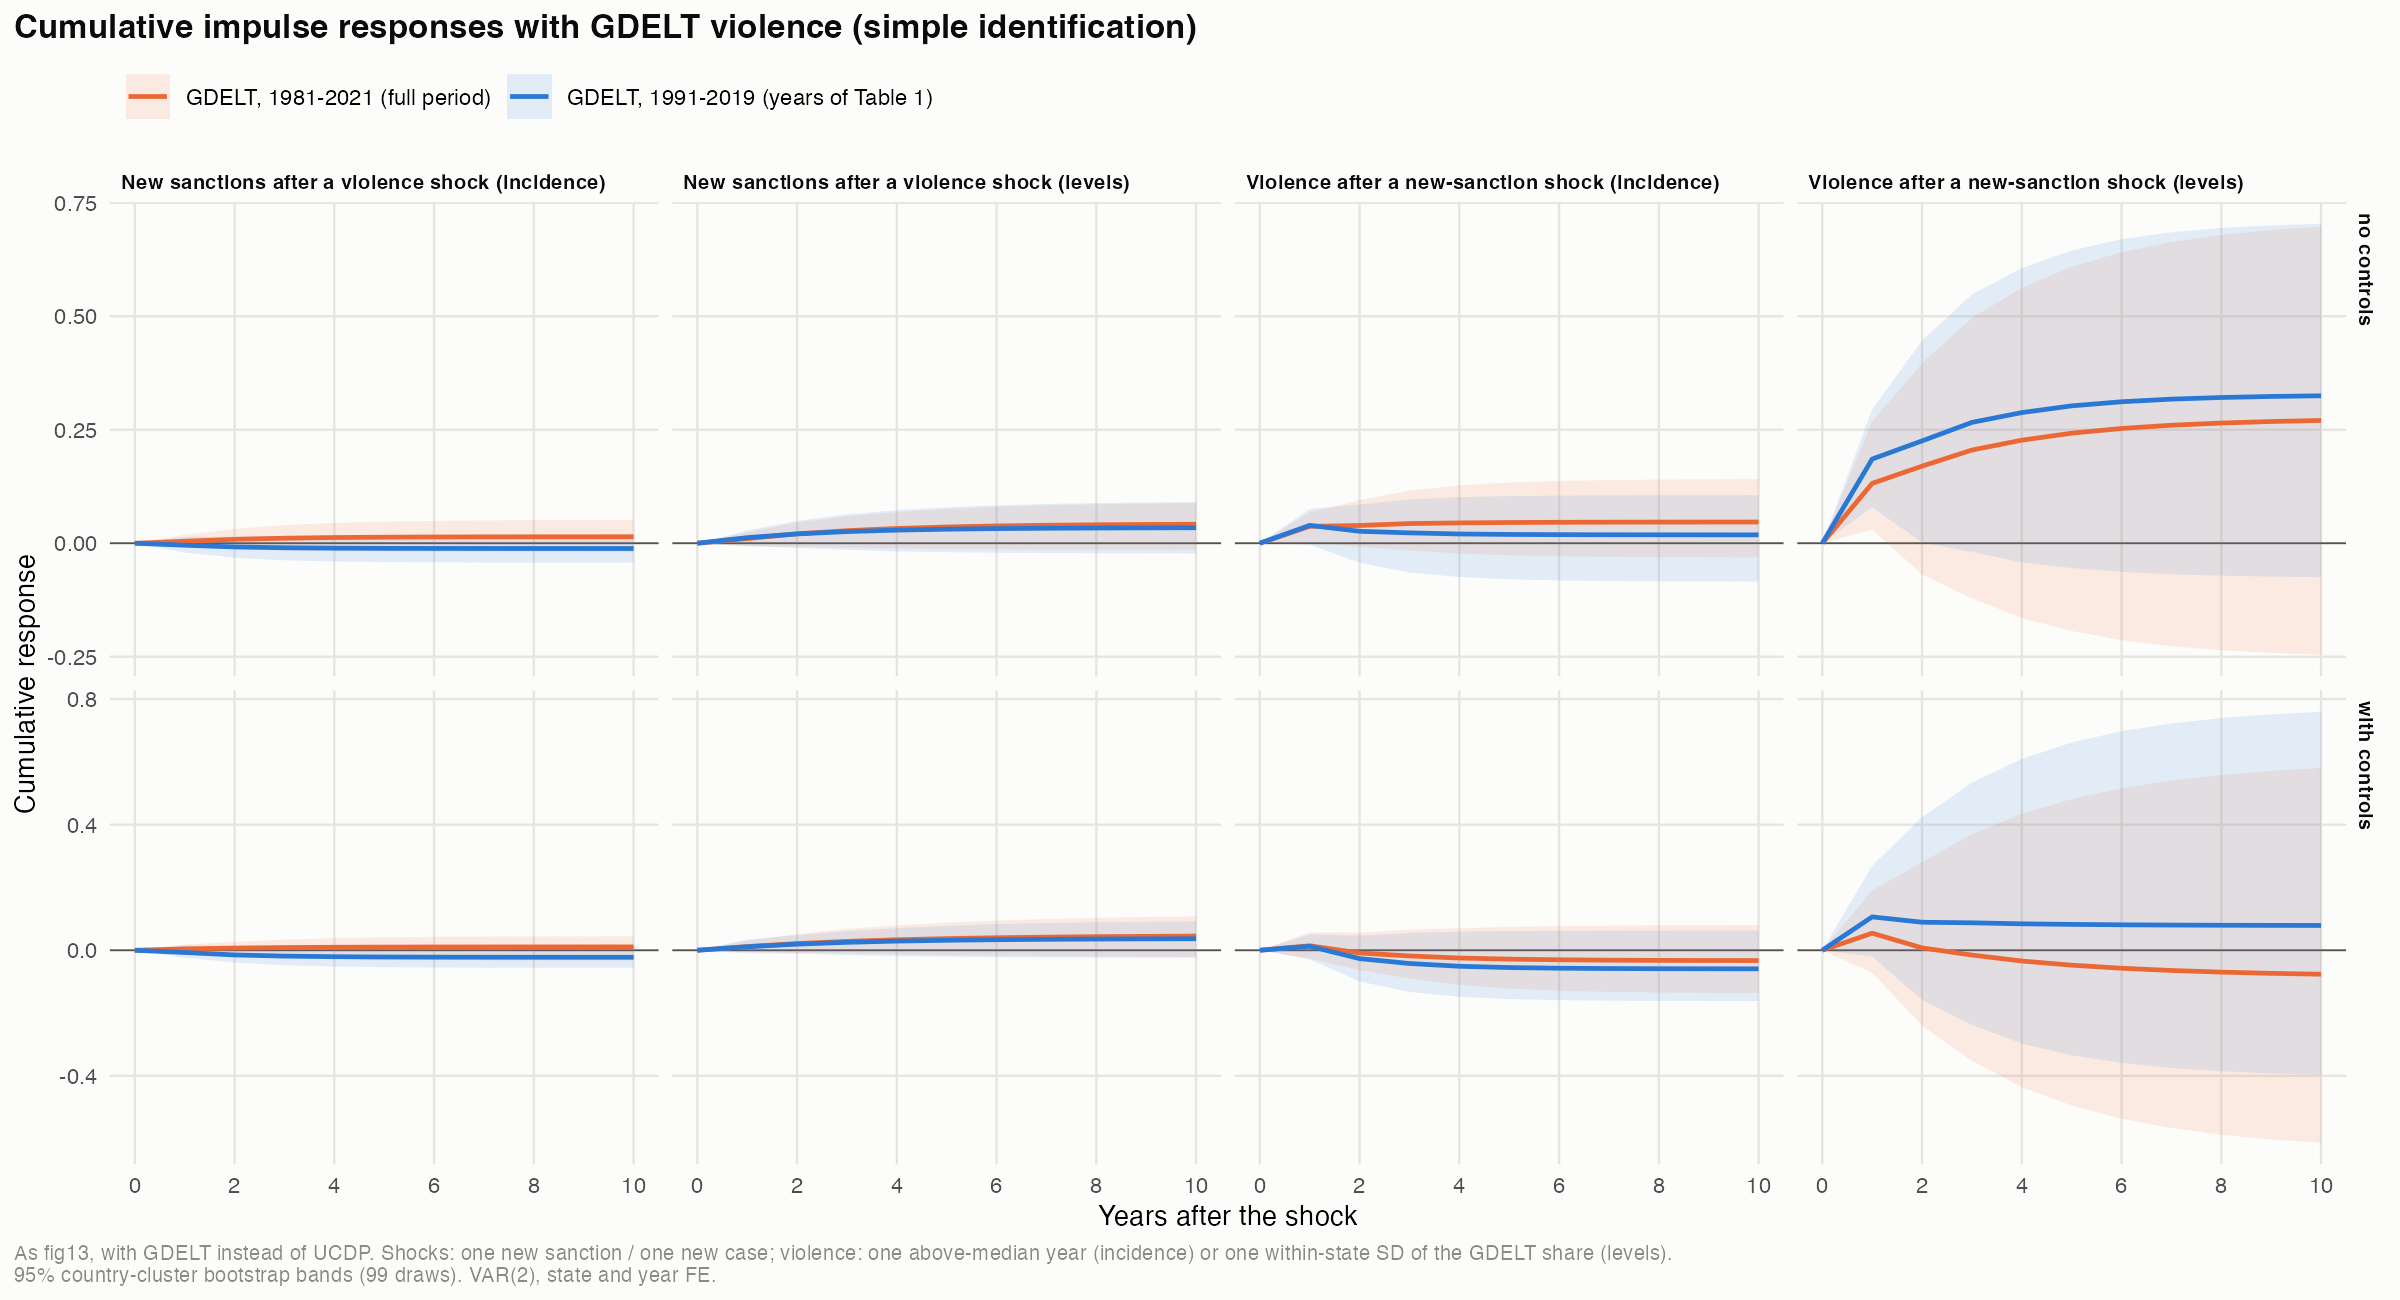
\includegraphics[width=\textwidth]{fig14_gdelt_cumulative_irf.png}
\caption{Cumulative impulse responses with GDELT violence}
\label{fig:gdeltirf}
\end{figure}

\begin{figure}[htbp]
\centering
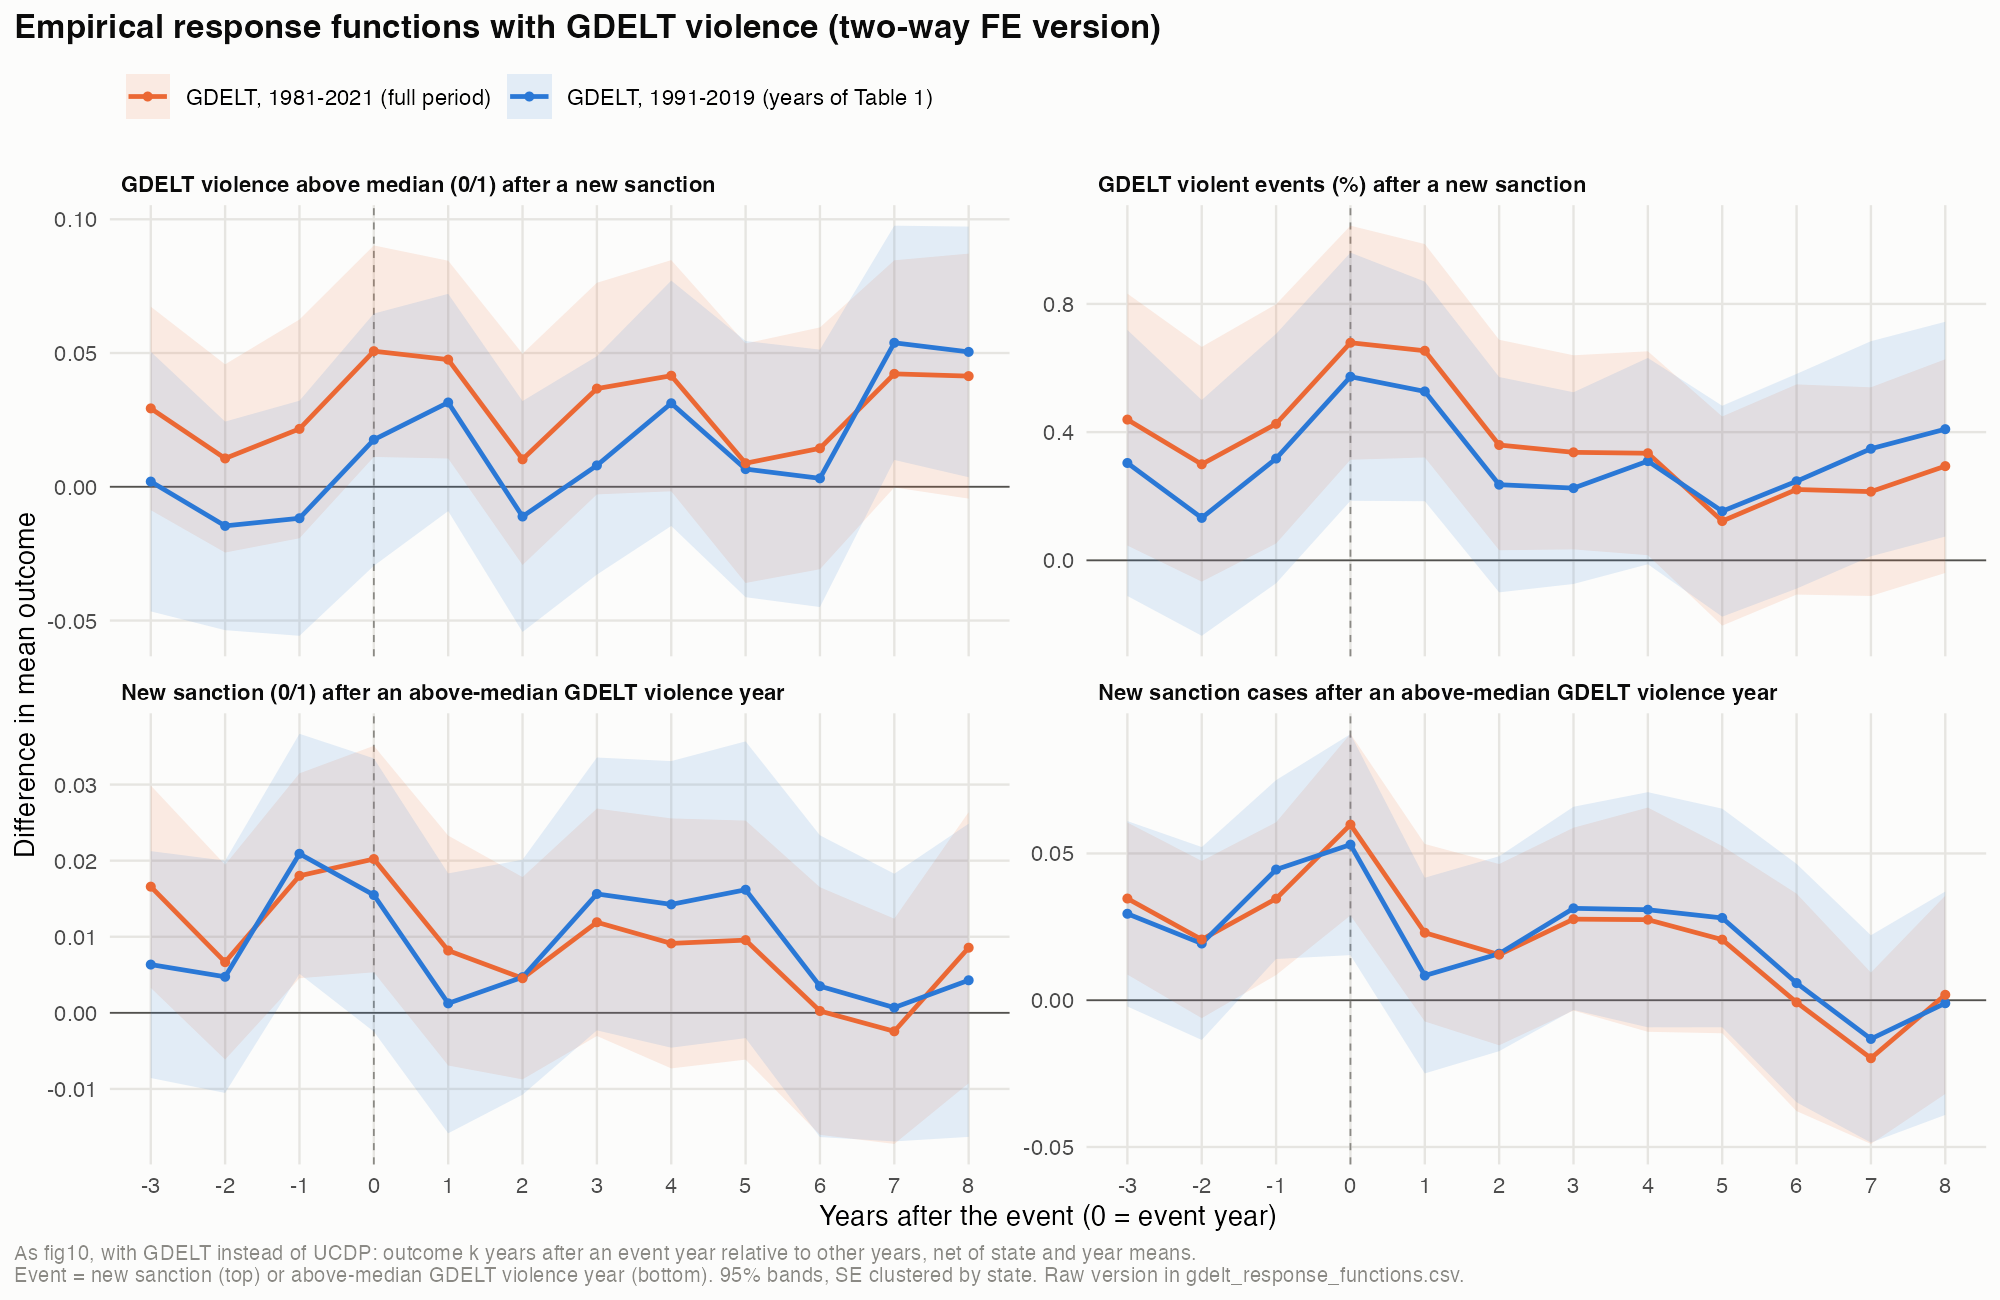
\includegraphics[width=\textwidth]{fig15_gdelt_response_functions.png}
\caption{Response functions with GDELT violence}
\label{fig:gdeltresponse}
\end{figure}

\subsection{Controls and the Yugoslav cases}
\label{sec:controls}
% NUMBERS: tab:controls, tab:yugoslavia (run 2026-10-23 16:50)

\paragraph{Which control drives what (decision D8).} Panels A and B of Table~\ref{tab:granger} differ in two
ways: the controls, and the sample (174 instead of 197 states, because V-Dem does not cover microstates).
Table~\ref{tab:controls} separates the two by estimating every version on one common sample.
\begin{itemize}[leftmargin=*]
\item \emph{The sample does not matter:} fixed effects only on the 174-state sample give the same results as on the
  full sample.
\item \emph{Sanctions $\rightarrow$ violence, incidence:} the negative sum appears only with the stock of sanctions
  in force in $t-1$ ($-0.032$ alone, $-0.036$ with all controls); with fixed effects only, GDP growth, democracy, or
  the stock dated $t-3$, the sum is between $-0.009$ and $0.000$. The stock in $t-1$ equals the stock in $t-3$ plus
  the new cases of $t-1$ and $t-2$ (minus lifted cases): it contains the regressors being tested. Conditioning on
  it changes what the sanction lags measure --- a new case for a given number of cases still in force, identified
  mainly from cases that were lifted again quickly. This is a bad control, not evidence of an effect.
\item \emph{Sanctions $\rightarrow$ violence, levels:} $-0.035$ to $-0.050$, significant at 5\% in every version.
\item \emph{Violence $\rightarrow$ sanctions:} incidence significant in every version; levels lose significance only
  with GDP growth.
\end{itemize}
Consequence: fixed effects only as the main specification; if a stock control is wanted, it should be dated $t-3$.

\begin{table}[htbp]
\centering
\small
\caption{Same-sample control check (decision D8)}
\label{tab:controls}
\begin{threeparttable}
\begin{tabular}{lcccc}
\toprule
 & \multicolumn{2}{c}{Incidence} & \multicolumn{2}{c}{Levels} \\
\cmidrule(lr){2-3}\cmidrule(lr){4-5}
Controls & $\chi^2(2)$ & Sum (SE) & $\chi^2(2)$ & Sum (SE) \\
\midrule
\multicolumn{5}{l}{\textit{Sanctions $\rightarrow$ violence}} \\
\quad FE only & 4.58 & $-$0.000 (0.017) & 7.05$^{**}$ & $-$0.035 (0.025) \\
\quad Sanction stock, $t-1$ & 6.88$^{**}$ & $-$0.032 (0.020) & 7.42$^{**}$ & $-$0.041 (0.025) \\
\quad Sanction stock, $t-3$ & 5.29$^{*}$ & $-$0.000 (0.017) & 7.02$^{**}$ & $-$0.036 (0.026) \\
\quad GDP growth & 4.15 & $-$0.005 (0.018) & 7.52$^{**}$ & $-$0.044 (0.026) \\
\quad Democracy & 4.46 & $-$0.005 (0.018) & 7.08$^{**}$ & $-$0.036 (0.026) \\
\quad All controls (Table~\ref{tab:granger}) & 7.12$^{**}$ & $-$0.036 (0.020) & 7.96$^{**}$ & $-$0.050 (0.026) \\
\quad All controls, stock $t-3$ & 4.80$^{*}$ & $-$0.009 (0.018) & 7.55$^{**}$ & $-$0.045 (0.027) \\
\quad FE only, full sample (197 states) & 5.01$^{*}$ & 0.002 (0.017) & 7.14$^{**}$ & $-$0.035 (0.025) \\
\midrule
\multicolumn{5}{l}{\textit{Violence $\rightarrow$ sanctions}} \\
\quad FE only & 9.04$^{**}$ & 0.067 (0.023) & 6.76$^{**}$ & 0.043 (0.020) \\
\quad Sanction stock, $t-1$ & 9.16$^{**}$ & 0.068 (0.023) & 7.79$^{**}$ & 0.049 (0.020) \\
\quad Sanction stock, $t-3$ & 11.54$^{***}$ & 0.076 (0.022) & 7.97$^{**}$ & 0.050 (0.020) \\
\quad GDP growth & 7.25$^{**}$ & 0.060 (0.023) & 2.97 & 0.031 (0.020) \\
\quad Democracy & 7.52$^{**}$ & 0.061 (0.022) & 5.73$^{*}$ & 0.037 (0.020) \\
\quad All controls (Table~\ref{tab:granger}) & 6.25$^{**}$ & 0.056 (0.022) & 2.79 & 0.030 (0.020) \\
\quad All controls, stock $t-3$ & 7.81$^{**}$ & 0.063 (0.022) & 2.88 & 0.031 (0.020) \\
\quad FE only, full sample (197 states) & 9.86$^{***}$ & 0.070 (0.022) & 7.30$^{**}$ & 0.045 (0.020) \\
\bottomrule
\end{tabular}
\begin{tablenotes}[flushleft]\footnotesize
\item \textit{Notes:} FE-OLS VAR(2) with state and year fixed effects as in Table~\ref{tab:granger}; all rows except the last on one common sample (4,888 observations, 174 states: all controls available, including the sanction stock in $t-3$). Sanction stock in $t-1$ = cases in force in $t-1$; it equals the stock in $t-3$ plus the new cases of $t-1$ and $t-2$ (minus lifted cases), i.e.\ it contains the tested sanction lags. Sum = sum of the two cross-lag coefficients. Standard errors clustered by state. $^{*}p<0.1$, $^{**}p<0.05$, $^{***}p<0.01$.
\end{tablenotes}
\end{threeparttable}
\end{table}


\paragraph{Yugoslav sanction cases.} GSDB cases against Yugoslavia are attributed to its successor states, so one
case can appear as a new case in several states in the same year. A period dummy for these states (used in earlier
versions) is almost fully absorbed by the state fixed effects and does not address this; it was dropped from the
controls. Table~\ref{tab:yugoslavia} instead drops the eight ex-Yugoslav states, or treats them as a single cluster.
Senders' reaction to violence is unaffected. The sanctions$\rightarrow$violence effect is somewhat weaker without
these states (levels, fixed effects only: $-0.024$, $p=0.080$; with controls $-0.040$, $p=0.044$), so part of it comes
from the Yugoslav cases; clustering them together changes the $p$-values little.

\begin{table}[htbp]
\centering
\footnotesize
\caption{Robustness: attribution of Yugoslav sanction cases}
\label{tab:yugoslavia}
\begin{threeparttable}
\begin{tabular}{llcccc}
\toprule
 & & \multicolumn{2}{c}{Incidence} & \multicolumn{2}{c}{Levels} \\
\cmidrule(lr){3-4}\cmidrule(lr){5-6}
Version & Controls & $\chi^2(2)$ & Sum (SE) & $\chi^2(2)$ & Sum (SE) \\
\midrule
\multicolumn{6}{l}{\textit{Sanctions $\rightarrow$ violence}} \\
\quad Main (Table~\ref{tab:granger}) & FE only & 5.01$^{*}$ & 0.002 (0.017) & 7.14$^{**}$ & $-$0.035 (0.025) \\
\quad Main (Table~\ref{tab:granger}) & with controls & 7.27$^{**}$ & $-$0.035 (0.020) & 8.08$^{**}$ & $-$0.050 (0.025) \\
\quad Without ex-Yugoslav states & FE only & 3.96 & 0.010 (0.016) & 5.06$^{*}$ & $-$0.024 (0.022) \\
\quad Without ex-Yugoslav states & with controls & 5.30$^{*}$ & $-$0.029 (0.019) & 6.25$^{**}$ & $-$0.040 (0.024) \\
\quad Ex-Yugoslav states one cluster & FE only & 4.91$^{*}$ & 0.002 (0.017) & 5.35$^{*}$ & $-$0.035 (0.025) \\
\quad Ex-Yugoslav states one cluster & with controls & 6.68$^{**}$ & $-$0.035 (0.020) & 6.35$^{**}$ & $-$0.050 (0.025) \\
\midrule
\multicolumn{6}{l}{\textit{Violence $\rightarrow$ sanctions}} \\
\quad Main (Table~\ref{tab:granger}) & FE only & 9.86$^{***}$ & 0.070 (0.022) & 7.30$^{**}$ & 0.045 (0.020) \\
\quad Main (Table~\ref{tab:granger}) & with controls & 6.22$^{**}$ & 0.056 (0.022) & 2.82 & 0.031 (0.019) \\
\quad Without ex-Yugoslav states & FE only & 9.13$^{**}$ & 0.069 (0.023) & 6.30$^{**}$ & 0.046 (0.021) \\
\quad Without ex-Yugoslav states & with controls & 5.92$^{*}$ & 0.055 (0.023) & 2.68 & 0.033 (0.020) \\
\quad Ex-Yugoslav states one cluster & FE only & 9.88$^{***}$ & 0.070 (0.022) & 7.35$^{**}$ & 0.045 (0.020) \\
\quad Ex-Yugoslav states one cluster & with controls & 6.24$^{**}$ & 0.056 (0.022) & 2.83 & 0.031 (0.019) \\
\bottomrule
\end{tabular}
\begin{tablenotes}[flushleft]\footnotesize
\item \textit{Notes:} FE-OLS VAR(2) as in Table~\ref{tab:granger}. GSDB cases against Yugoslavia are attributed to its successor states, so one case can appear in several states. Ex-Yugoslav states: Yugoslavia/FRY, Serbia, Montenegro, Macedonia, Croatia, Bosnia-Herzegovina, Kosovo, Slovenia. \emph{One cluster}: standard errors clustered by state, except that the ex-Yugoslav states form a single cluster. $^{*}p<0.1$, $^{**}p<0.05$, $^{***}p<0.01$.
\end{tablenotes}
\end{threeparttable}
\end{table}


\subsection{Planned checks}
\begin{itemize}[leftmargin=*]
\item Leave-one-country-out estimates and the most influential sanction events.
\item Bias-corrected heterogeneous Granger test \citep{juodis2021} on the balanced panel (167 states).
\item Driscoll--Kraay standard errors.
\item Time aggregation (two- and three-year periods), as in \citet[Table 3]{jaeger2008}.
\item Splits: sender (UN, EU, US), sanction type (arms embargoes), objective (conflict-related), period.
\item Anticipation proxy (GDELT threats and coercion), analogous to \citet[Table 4]{jaeger2008}.
\item Sample to 2023; effects of sanction \emph{lifting}.
\end{itemize}

% =============================================================================
\section{Extension (not part of the base case): LP-DiD event study}
\label{sec:extension}
% NUMBERS: Table 11 (run 2026-10-22)

The response functions of Section~\ref{sec:results} compare event years with \emph{all} other years. A modern
alternative is the local-projection difference-in-differences estimator of \citet{dube2023}, which compares
states with a new event to a set of ``clean'' control states and is designed for treatments that switch on and
off. This section describes what it estimates, what it shows, and how it relates to the VAR. It is kept separate
from the base case because it answers a different question and its role in the paper is not yet decided.

\subsection{Design}
For each horizon $h=-3,\dots,8$ we estimate
\begin{equation}
y_{i,t+h}-y_{i,t-1} = \beta_h D_{it} + \gamma_h' (y_{i,t-1},\, y_{i,t-2}) + \tau_t + e_{it},
\label{eq:lpdid}
\end{equation}
on two groups of state-years only. \emph{Treated}: an event in $t$ and none in the three previous years.
\emph{Clean controls}: no event in $t$ and none in the three previous years. In the sanction direction the event
is a new sanction; in the reverse direction it is a conflict \emph{onset} (a conflict year after three peaceful
years), because conflict comes in spells. The outcome is the change relative to the year before the event, so
time-invariant state differences drop out without state fixed effects; year effects absorb common shocks; the two
lagged outcomes (used for $h\geq 0$) control for selection on recent violence, as in Dube et al.'s democracy
application. The pre-event coefficients ($h=-3,-2$) are estimated without these controls, since otherwise
$h=-2$ would be zero by construction; they test whether treated and control states were already moving
differently before the year preceding the event.

Restricting comparisons to clean controls avoids the problem that two-way fixed-effects and panel local-projection
regressions with on/off treatments implicitly use already-treated states as controls, which can bias them, even in
sign \citep{dechaisemartin2026}. Because the regression has no state fixed effects, the Nickell bias of panel local
projections with fixed effects \citep{mei2026} does not arise in the same form.

\begin{table}[htbp]
\centering
\footnotesize\setlength{\tabcolsep}{4pt}
\caption{LP-DiD event study (extension): change in the outcome relative to the year before the event}
\label{tab:lpdid}
\begin{threeparttable}
\begin{tabular}{lcccccc}
\toprule
 & \multicolumn{2}{c}{UCDP: after a new sanction} & \multicolumn{2}{c}{UCDP: after a conflict onset} & \multicolumn{2}{c}{GDELT, 1991--2019} \\
\cmidrule(lr){2-3}\cmidrule(lr){4-5}\cmidrule(lr){6-7}
Horizon $h$ & \makecell{Conflict\\(0/1)} & \makecell{log deaths\\per 100k} & \makecell{New sanction\\(0/1)} & \makecell{New\\cases} & \makecell{Violent share (\%)\\after sanction} & \makecell{New sanction\\after onset} \\
\midrule
-3 & $-$0.002 & $-$0.020 & 0.004 & 0.032 & 0.307 & $-$0.040 \\
 & (0.019) & (0.035) & (0.036) & (0.067) & (0.233) & (0.024) \\
-2 & 0.012 & 0.004 & $-$0.005 & 0.002 & 0.043 & $-$0.050$^{**}$ \\
 & (0.017) & (0.034) & (0.038) & (0.063) & (0.169) & (0.023) \\
\midrule
0 & 0.086$^{***}$ & 0.230$^{***}$ & 0.128$^{***}$ & 0.427$^{***}$ & 0.812$^{***}$ & 0.010 \\
 & (0.019) & (0.054) & (0.036) & (0.142) & (0.179) & (0.019) \\
1 & 0.080$^{***}$ & 0.199$^{***}$ & 0.065$^{*}$ & 0.148$^{*}$ & 1.032$^{***}$ & $-$0.016 \\
 & (0.021) & (0.051) & (0.034) & (0.084) & (0.201) & (0.020) \\
2 & 0.063$^{***}$ & 0.119$^{**}$ & 0.124$^{***}$ & 0.261$^{***}$ & 0.710$^{***}$ & 0.010 \\
 & (0.021) & (0.048) & (0.041) & (0.099) & (0.180) & (0.021) \\
3 & 0.040$^{*}$ & 0.108$^{**}$ & 0.038 & 0.040 & 0.836$^{***}$ & $-$0.008 \\
 & (0.021) & (0.046) & (0.035) & (0.054) & (0.225) & (0.022) \\
5 & 0.033 & 0.103$^{**}$ & 0.107$^{***}$ & 0.253$^{**}$ & 0.586$^{***}$ & $-$0.007 \\
 & (0.023) & (0.044) & (0.041) & (0.115) & (0.214) & (0.018) \\
8 & 0.020 & 0.118$^{*}$ & 0.025 & 0.028 & 0.930$^{***}$ & 0.002 \\
 & (0.026) & (0.064) & (0.030) & (0.050) & (0.266) & (0.023) \\
\midrule
Treated events & 348 & 348 & 111 & 111 & 348 & 356 \\
\bottomrule
\end{tabular}
\begin{tablenotes}[flushleft]\footnotesize
\item \textit{Notes:} Coefficient on the treatment dummy in $y_{i,t+h}-y_{i,t-1} = \beta_h D_{it} + \gamma_h'(y_{i,t-1}, y_{i,t-2}) + \tau_t + e_{it}$ \citep{dube2023}, estimated on treated state-years (event in $t$, none in the three previous years) and clean controls (no event in $t$ and the three previous years); lagged outcomes only for $h\geq 0$; reference year $h=-1$. Conflict onset: conflict year after three years without conflict; GDELT violence onset: above-median year after three years at or below the median. GDELT columns 1991--2019. Standard errors clustered by state. $^{*}p<0.1$, $^{**}p<0.05$, $^{***}p<0.01$.
\end{tablenotes}
\end{threeparttable}
\end{table}


\subsection{Results}
Table~\ref{tab:lpdid} and Figure~\ref{fig:lpdid} summarise the estimates.
\begin{itemize}[leftmargin=*]
\item \textit{Pre-trends.} In the UCDP data, treated and clean-control states move in parallel before the event in
  both directions (all pre-event coefficients small and insignificant).
\item \textit{Violence after a new sanction} (348 events). Relative to clean controls, the conflict probability
  rises by 8.6 percentage points in the sanction year and remains 6.3 points higher two years later; log deaths
  per capita rise by 0.23 and stay 0.10--0.12 higher up to eight years later (marginally significant at $h=8$).
\item \textit{New sanctions after a conflict onset} (111 events). The probability of a new sanction rises by 12.8
  percentage points in the onset year, with further increases at $h=2$ and $h=5$: senders react quickly and keep
  reacting while the conflict lasts.
\item \textit{GDELT.} The violent share of reported events is 0.8--1.1 percentage points higher in the years after a
  new sanction, with flat pre-trends. After a GDELT violence onset there is no sanction response, but the
  pre-trends are significantly negative, so this comparison is not credible with the median-based onset
  definition (Figure~\ref{fig:lpdidgdelt}).
\end{itemize}

\subsection{How the event study relates to the VAR}
At first sight the event study contradicts the VAR: violence is \emph{higher} after a sanction here, while the VAR
finds a \emph{lower} conflict probability two years after a sanction. The two estimates condition on different
things.
\begin{enumerate}[leftmargin=*]
\item \textbf{Reference point.} The event study measures violence relative to the year \emph{before} the sanction
  ($t-1$). In the violence equation of the VAR, the coefficient on a sanction in $t-2$ is estimated conditional on
  violence in $t-2$ and $t-1$ --- that is, on violence in the \emph{sanction year} itself and the year after. The VAR therefore asks whether violence
  after the sanction year is lower than the sanction-year level and its usual persistence predict; the event study
  asks whether it is higher than before the sanction. Both can be true at the same time: sanctions come with an
  escalation, after which violence declines faster than usual (VAR) but stays above its pre-sanction level
  (event study). The response functions (Figure~\ref{fig:response}) show exactly this shape.
\item \textbf{Within-year timing.} The jump at $h=0$ mixes the escalation that led to the sanction with any effect
  of the sanction itself. Flat pre-trends only show that treated states were not on a different path up to $t-1$;
  they cannot rule out that the sanction responded to violence earlier in the same year. This is the same
  identification problem as the ordering of the impulse responses, and the event study does not solve it.
\item \textbf{Total versus partial effect.} The event study measures everything that follows a new sanction
  episode, including follow-up sanctions (P(new sanction $|$ new sanction last year) $=0.30$) and the
  conflict dynamics already under way. The VAR isolates the response to a sanction innovation holding the past of
  both variables fixed.
\item \textbf{Comparison group.} Clean controls are states without any new sanction for four years; senders did
  not target them, and they may differ systematically from targeted states (for example, be more peaceful). The year effects and lagged outcomes reduce but do not
  remove this selection; in the reverse direction, onsets of conflict are compared with persistently peaceful
  states.
\end{enumerate}
The direction of reverse causality (violence $\rightarrow$ sanctions) is the robust common finding: sanctions
follow conflict onsets in the event study, Granger-follow violence in the VAR, and rise around conflict years in
the response functions.

\subsection{Assessment and possible next steps}
\textit{Strengths:} transparent, model-free comparison with a clear treated/control structure; robust to the
negative-weighting problem of fixed-effects regressions; explicit pre-trend test; easy to communicate.
\textit{Weaknesses for our question:} it cannot separate within-year reverse causality, it measures a total
effect that includes follow-up sanctions, and its controls are selected on not being sanctioned.
Possible refinements, if it enters the paper:
\begin{itemize}[leftmargin=*]
\item Condition on the escalation: compare sanctioned states with clean controls that had the same violence in the
  event year (i.e.\ add $y_{it}$ or match on conflict status in $t$), which brings the estimand close to the VAR's.
\item Restrict to conflict-prone states (in conflict in $t-1$), the subsample where sanctions are typically
  imposed (decision D7 in the analysis plan).
\item Separate sanctions by objective (conflict-related) and by type (arms embargoes), where an effect on violence
  is most plausible.
\item Report the equally-weighted (reweighted) version of \citet{dube2023} and vary the clean-control window.
\end{itemize}
\todo{decide: (a) appendix as a complement to the response functions, (b) main-text robustness section, or
(c) drop.}

\begin{figure}[htbp]
\centering
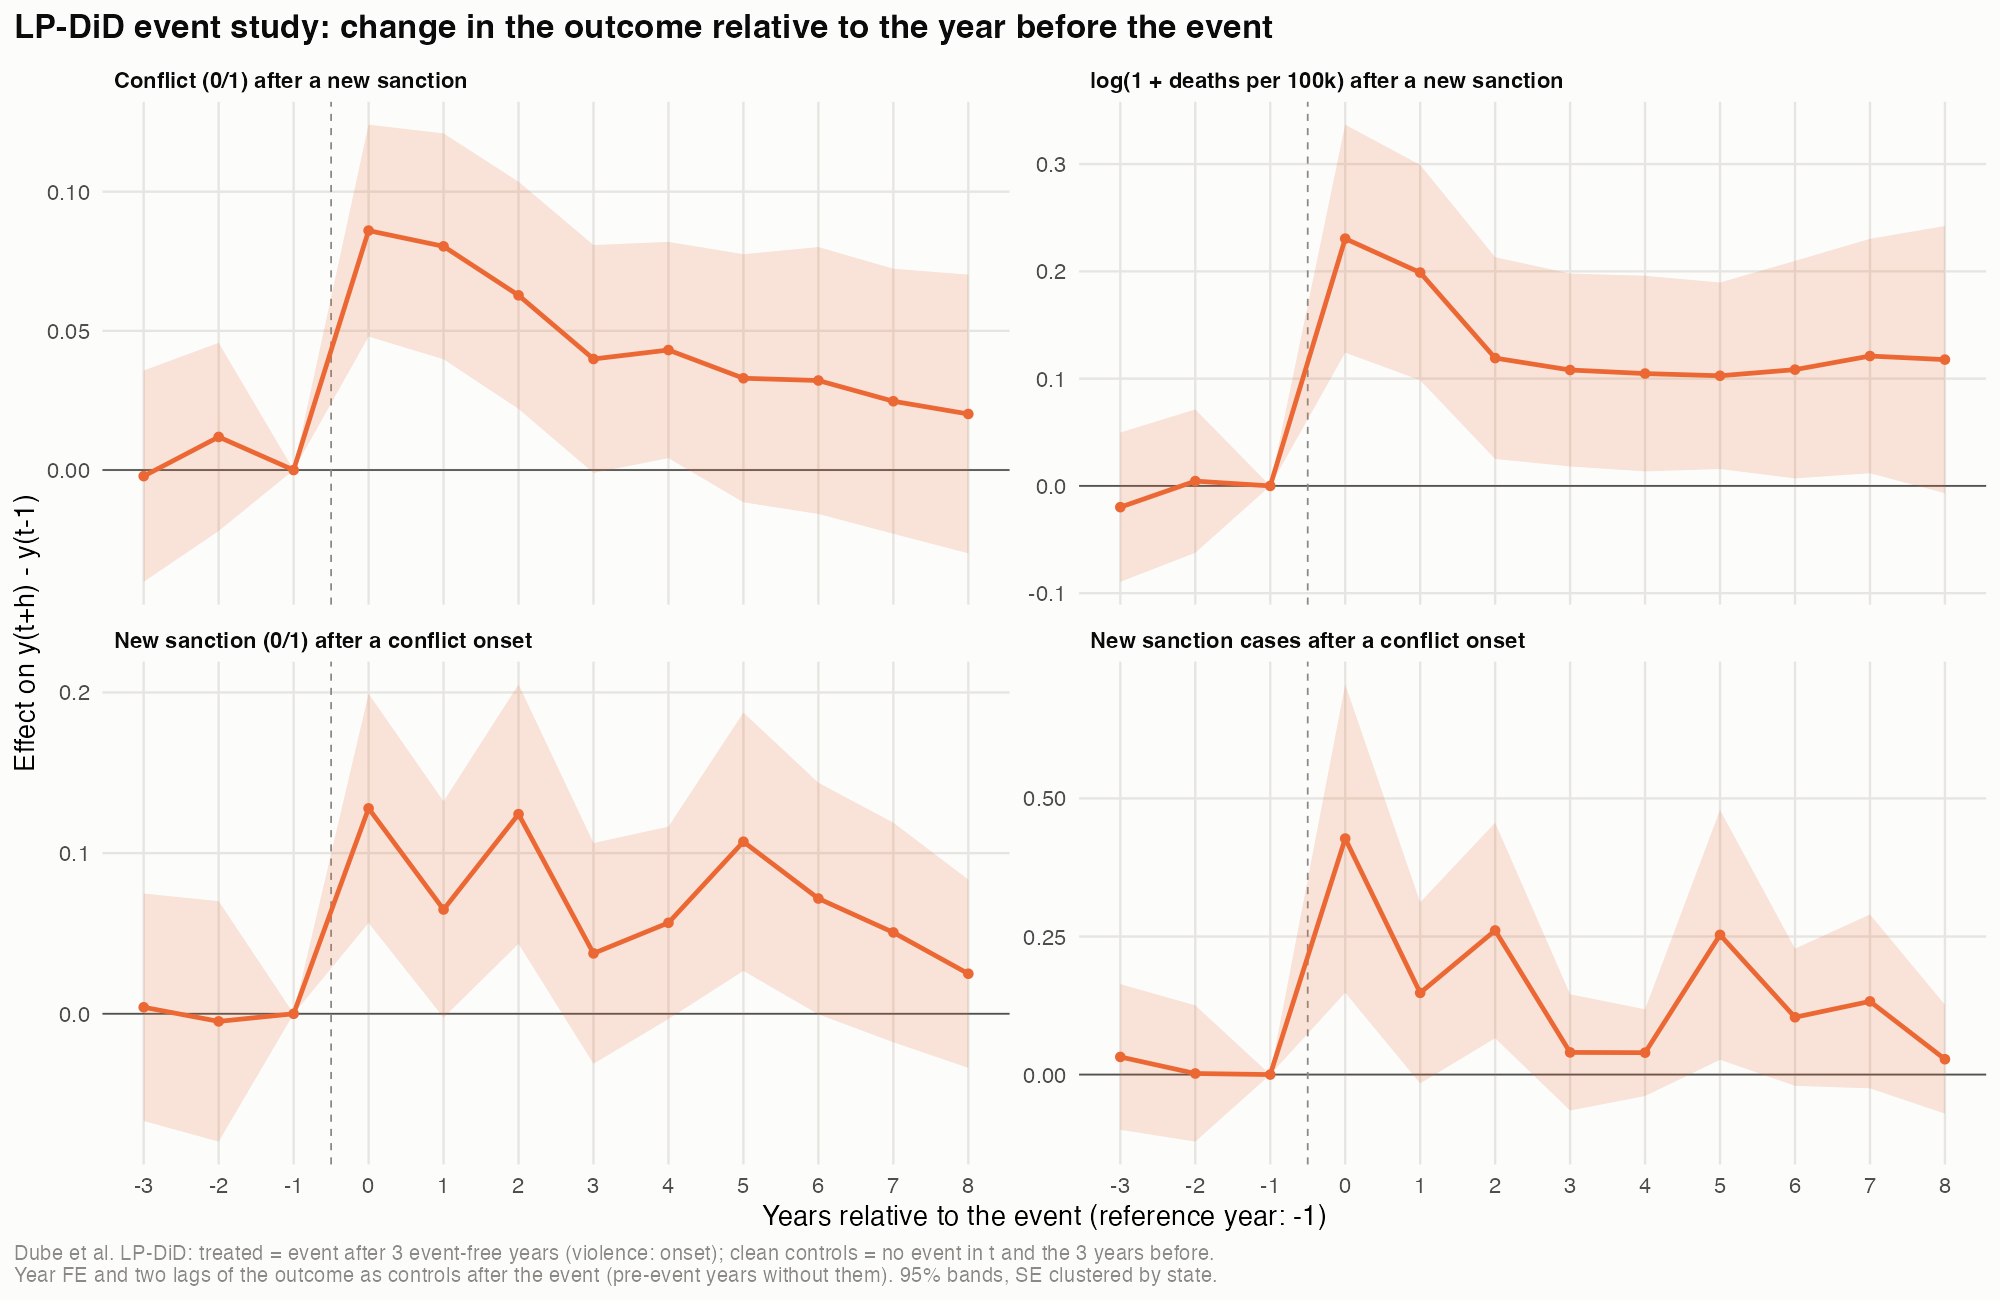
\includegraphics[width=\textwidth]{fig11_lpdid_event_study.png}
\caption{LP-DiD event study with UCDP violence (extension)}
\label{fig:lpdid}
\end{figure}

\begin{figure}[htbp]
\centering
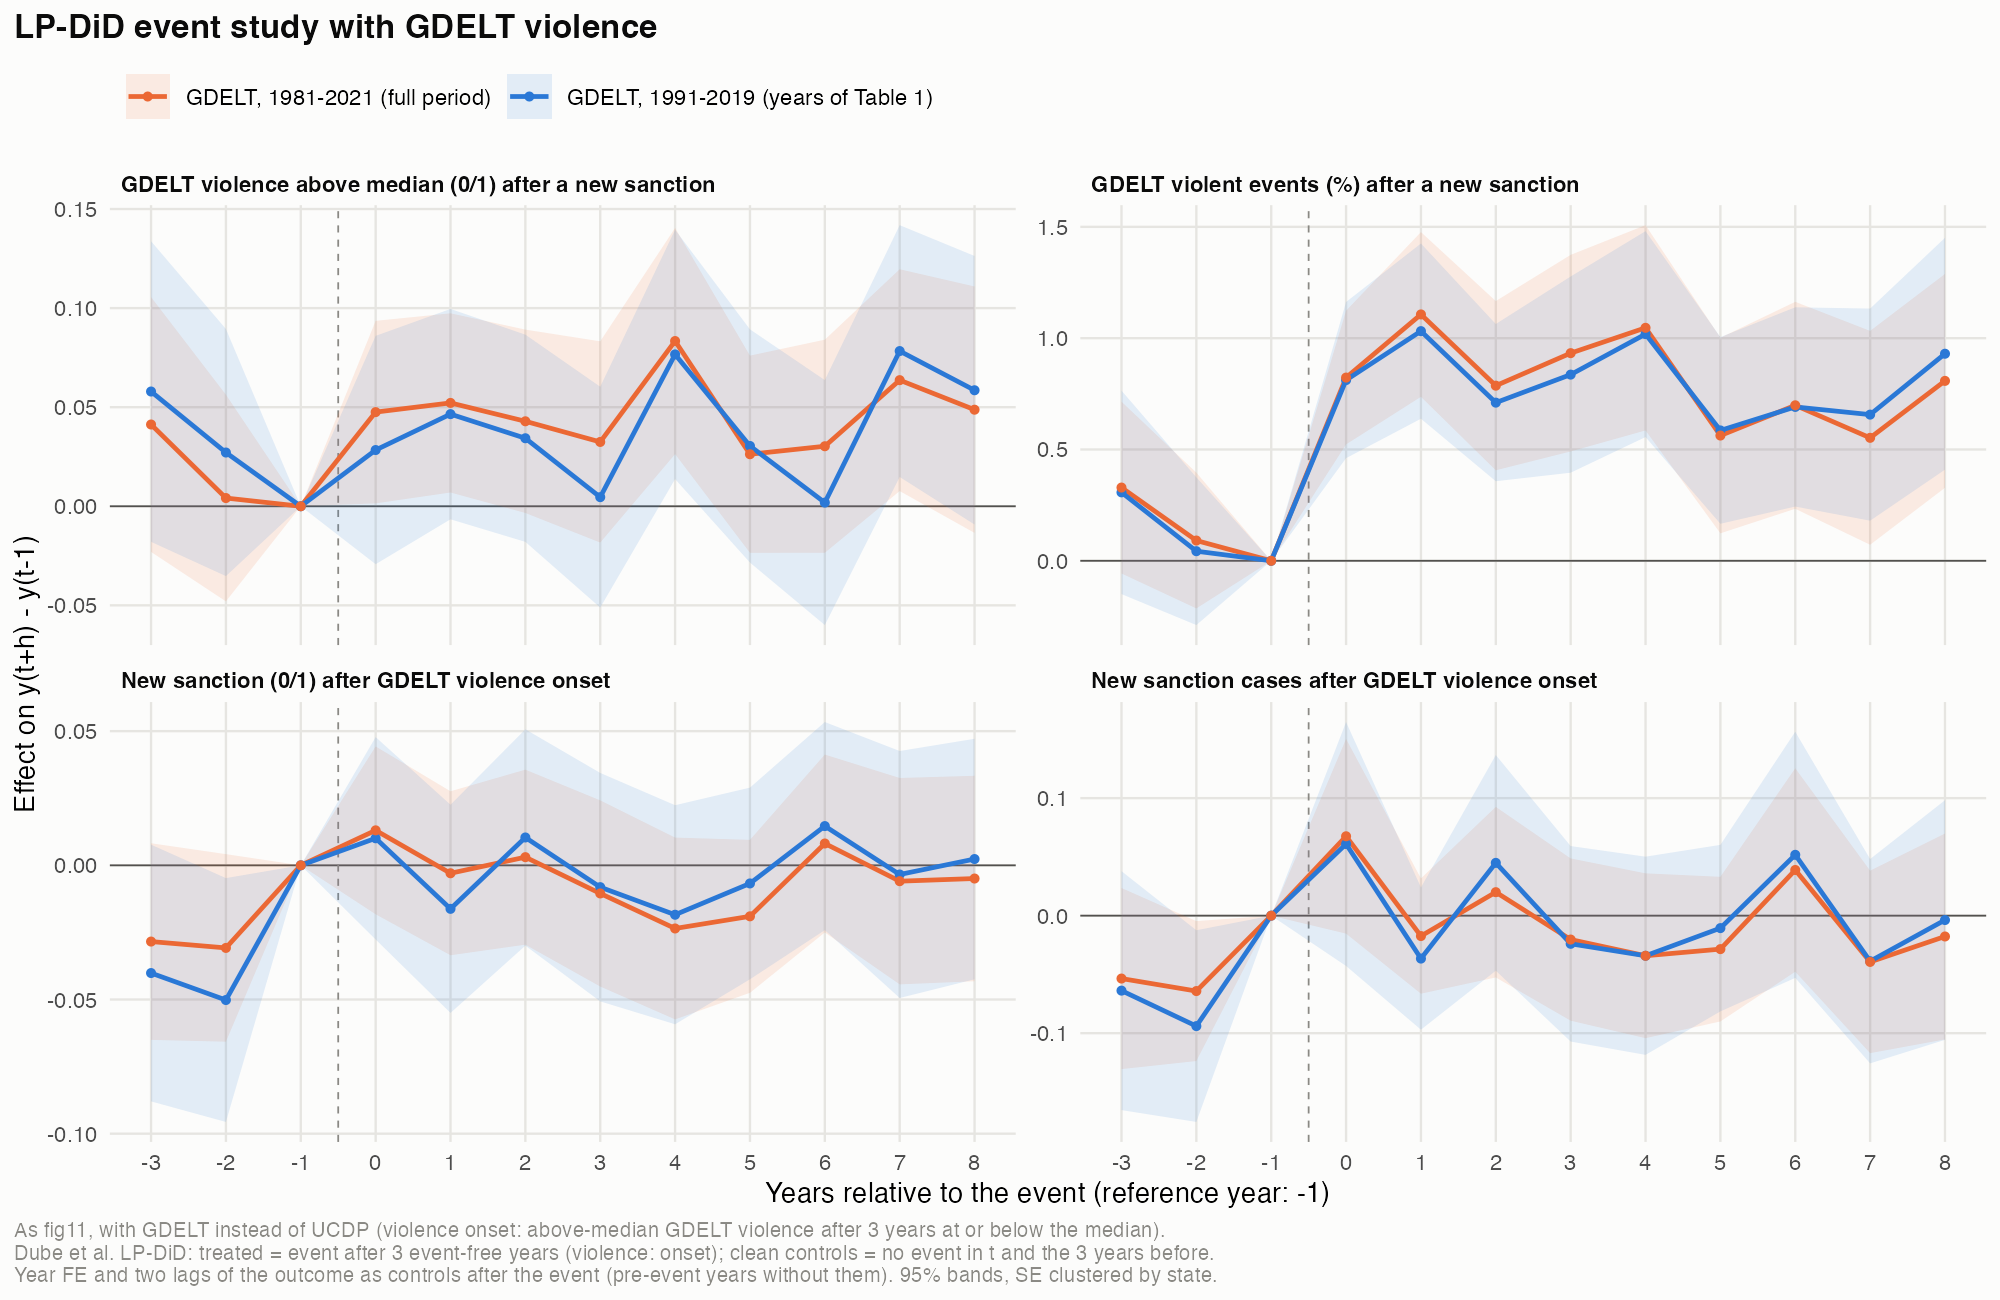
\includegraphics[width=\textwidth]{fig16_gdelt_lpdid_event_study.png}
\caption{LP-DiD event study with GDELT violence (extension)}
\label{fig:lpdidgdelt}
\end{figure}

% =============================================================================
\section{Discussion and next steps}
\label{sec:discussion}

\begin{enumerate}[leftmargin=*]
\item \textbf{Main specification (D8).} Fixed effects only. The only result that needs the controls --- the
  incidence effect of sanctions on violence --- comes from the sanction stock in $t-1$, which contains the tested
  lags (Table~\ref{tab:controls}); the violence$\rightarrow$sanctions result is weakened by GDP growth, plausibly a
  bad control. Controls (with the stock dated $t-3$) as robustness.
\item \textbf{Within-year timing.} The sign of the sanction effect depends on whether sanctions can affect
  violence in the year they are imposed. Monthly data (UCDP GED events and sanction announcement dates) would
  resolve this and bring the design closer to the daily data of \citet{jaeger2008}.
\item \textbf{Measurement.} A stricter GDELT incidence definition (top quartile, mass-violence events).
\item \textbf{Functional form.} Logit, PPML and raw-deaths (capped) versions confirm both directions
  (Section~\ref{sec:robustness}); no further work needed here beyond a bias-corrected logit.
\item \textbf{Interpretation.} Rather than a symmetric cycle of violence, the evidence so far suggests that senders
  respond to violence, while sanctions are followed by somewhat fewer deaths two years later --- partly driven by
  the Yugoslav cases and with a sign that depends on timing assumptions --- but not by a lower probability of
  conflict, and possibly by more low-level violence.
\end{enumerate}

\paperonly{conclusion.}

% =============================================================================
\clearpage
\bibliographystyle{plainnat}
\bibliography{references}

% =============================================================================
\clearpage
\appendix
\section{Additional tables and figures}

\begin{table}[htbp]
\centering
\footnotesize
\caption{Reaction functions (FE-OLS): all coefficients}
\label{tab:coefficients}
\begin{threeparttable}
\begin{tabular}{lcccc}
\toprule
 & \multicolumn{2}{c}{Sender equation} & \multicolumn{2}{c}{Violence equation} \\
\cmidrule(lr){2-3}\cmidrule(lr){4-5}
Dependent variable & New sanction & New cases & Conflict & log deaths \\
\midrule
\multicolumn{5}{l}{\textit{A. With lagged controls}} \\
\quad Violence, $t-1$ & 0.029$^{*}$ & 0.028 & 0.352$^{***}$ & 0.585$^{***}$ \\
 & (0.017) & (0.024) & (0.030) & (0.046) \\
\quad Violence, $t-2$ & 0.027 & 0.002 & 0.133$^{***}$ & 0.062 \\
 & (0.018) & (0.023) & (0.028) & (0.039) \\
\quad New sanctions, $t-1$ & 0.130$^{***}$ & 0.086$^{***}$ & $-$0.000 & $-$0.007 \\
 & (0.018) & (0.020) & (0.013) & (0.015) \\
\quad New sanctions, $t-2$ & $-$0.016 & $-$0.007 & $-$0.035$^{***}$ & $-$0.044$^{***}$ \\
 & (0.017) & (0.015) & (0.013) & (0.016) \\
\quad Sanction stock, $t-1$ & $-$0.002 & $-$0.023$^{*}$ & 0.009$^{**}$ & 0.002 \\
 & (0.005) & (0.014) & (0.004) & (0.008) \\
\quad GDP growth, $t-1$ & $-$0.365$^{**}$ & $-$0.984$^{***}$ & $-$0.380$^{***}$ & $-$1.028$^{***}$ \\
 & (0.154) & (0.350) & (0.106) & (0.279) \\
\quad Democracy, $t-1$ & $-$0.155$^{**}$ & $-$0.433$^{***}$ & $-$0.111 & $-$0.054 \\
 & (0.060) & (0.150) & (0.077) & (0.111) \\
\midrule
\multicolumn{5}{l}{\textit{B. State and year FE only}} \\
\quad Violence, $t-1$ & 0.037$^{**}$ & 0.047$^{**}$ & 0.365$^{***}$ & 0.605$^{***}$ \\
 & (0.017) & (0.022) & (0.030) & (0.044) \\
\quad Violence, $t-2$ & 0.032$^{*}$ & $-$0.002 & 0.142$^{***}$ & 0.057 \\
 & (0.018) & (0.024) & (0.028) & (0.038) \\
\quad New sanctions, $t-1$ & 0.130$^{***}$ & 0.074$^{***}$ & 0.020$^{*}$ & 0.002 \\
 & (0.017) & (0.021) & (0.012) & (0.015) \\
\quad New sanctions, $t-2$ & $-$0.017 & $-$0.018 & $-$0.018 & $-$0.037$^{**}$ \\
 & (0.017) & (0.018) & (0.012) & (0.015) \\
\bottomrule
\end{tabular}
\begin{tablenotes}[flushleft]\footnotesize
\item \textit{Notes:} Bivariate panel VAR(2), equation by equation, state and year fixed effects, standard errors clustered by state in parentheses. Columns (1)--(2): new sanctions on lags of violence and of new sanctions; (3)--(4): violence on lags of violence and of new sanctions. 1991--2019. $^{*}p<0.1$, $^{**}p<0.05$, $^{***}p<0.01$.
\end{tablenotes}
\end{threeparttable}
\end{table}

\begin{table}[htbp]
\centering
\footnotesize
\caption{Granger tests for different lag structures: panel version of Jaeger and Paserman (2008), Table 2}
\label{tab:laggrid}
\begin{threeparttable}
\begin{tabular}{lcccc}
\toprule
 & \multicolumn{2}{c}{Violence $\rightarrow$ sanctions} & \multicolumn{2}{c}{Sanctions $\rightarrow$ violence} \\
\cmidrule(lr){2-3}\cmidrule(lr){4-5}
Lags (own, other) & Incidence & Levels & Incidence & Levels \\
\midrule
\multicolumn{5}{l}{\textit{A. With lagged controls}} \\
\quad (1, 1) & 0.011$^{**}$$^{\dagger}$ & 0.047$^{**}$$^{\dagger}$ & 0.861 & 0.361 \\
\quad (2, 1) & 0.010$^{**}$ & 0.048$^{**}$ & 0.977 & 0.608 \\
\quad (3, 1) & 0.012$^{**}$ & 0.048$^{**}$ & 0.985$^{\dagger}$ & 0.758 \\
\quad (1, 2) & 0.030$^{**}$ & 0.139 & 0.104 & 0.028$^{**}$ \\
\quad (2, 2) & 0.029$^{**}$ & 0.141 & 0.029$^{**}$ & 0.018$^{**}$ \\
\quad (3, 2) & 0.030$^{**}$ & 0.142 & 0.031$^{**}$ & 0.026$^{**}$$^{\dagger}$ \\
\quad (1, 3) & 0.067$^{*}$ & 0.242 & 0.210 & 0.051$^{*}$ \\
\quad (2, 3) & 0.065$^{*}$ & 0.243 & 0.066$^{*}$ & 0.029$^{**}$ \\
\quad (3, 3) & 0.070$^{*}$ & 0.249 & 0.064$^{*}$ & 0.041$^{**}$ \\
\midrule
\multicolumn{5}{l}{\textit{B. State and year FE only}} \\
\quad (1, 1) & 0.002$^{***}$$^{\dagger}$ & 0.005$^{***}$$^{\dagger}$ & 0.075$^{*}$ & 0.631 \\
\quad (2, 1) & 0.002$^{***}$ & 0.005$^{***}$ & 0.124 & 0.793 \\
\quad (3, 1) & 0.002$^{***}$ & 0.004$^{***}$ & 0.139$^{\dagger}$ & 0.853 \\
\quad (1, 2) & 0.006$^{***}$ & 0.015$^{**}$ & 0.176 & 0.081$^{*}$ \\
\quad (2, 2) & 0.006$^{***}$ & 0.014$^{**}$ & 0.102 & 0.031$^{**}$ \\
\quad (3, 2) & 0.005$^{***}$ & 0.014$^{**}$ & 0.101 & 0.040$^{**}$$^{\dagger}$ \\
\quad (1, 3) & 0.016$^{**}$ & 0.027$^{**}$ & 0.192 & 0.167 \\
\quad (2, 3) & 0.015$^{**}$ & 0.025$^{**}$ & 0.149 & 0.069$^{*}$ \\
\quad (3, 3) & 0.013$^{**}$ & 0.027$^{**}$ & 0.185 & 0.086$^{*}$ \\
\bottomrule
\end{tabular}
\begin{tablenotes}[flushleft]\footnotesize
\item \textit{Notes:} $p$-values of the Granger test (FE-OLS, clustered by state) for every combination of own lags and lags of the other variable; common sample with three lags of both variables (1992--2019), so that BIC is comparable. $^{\dagger}$ lowest BIC in the column. $^{*}p<0.1$, $^{**}p<0.05$, $^{***}p<0.01$.
\end{tablenotes}
\end{threeparttable}
\end{table}


\begin{figure}[htbp]
\centering
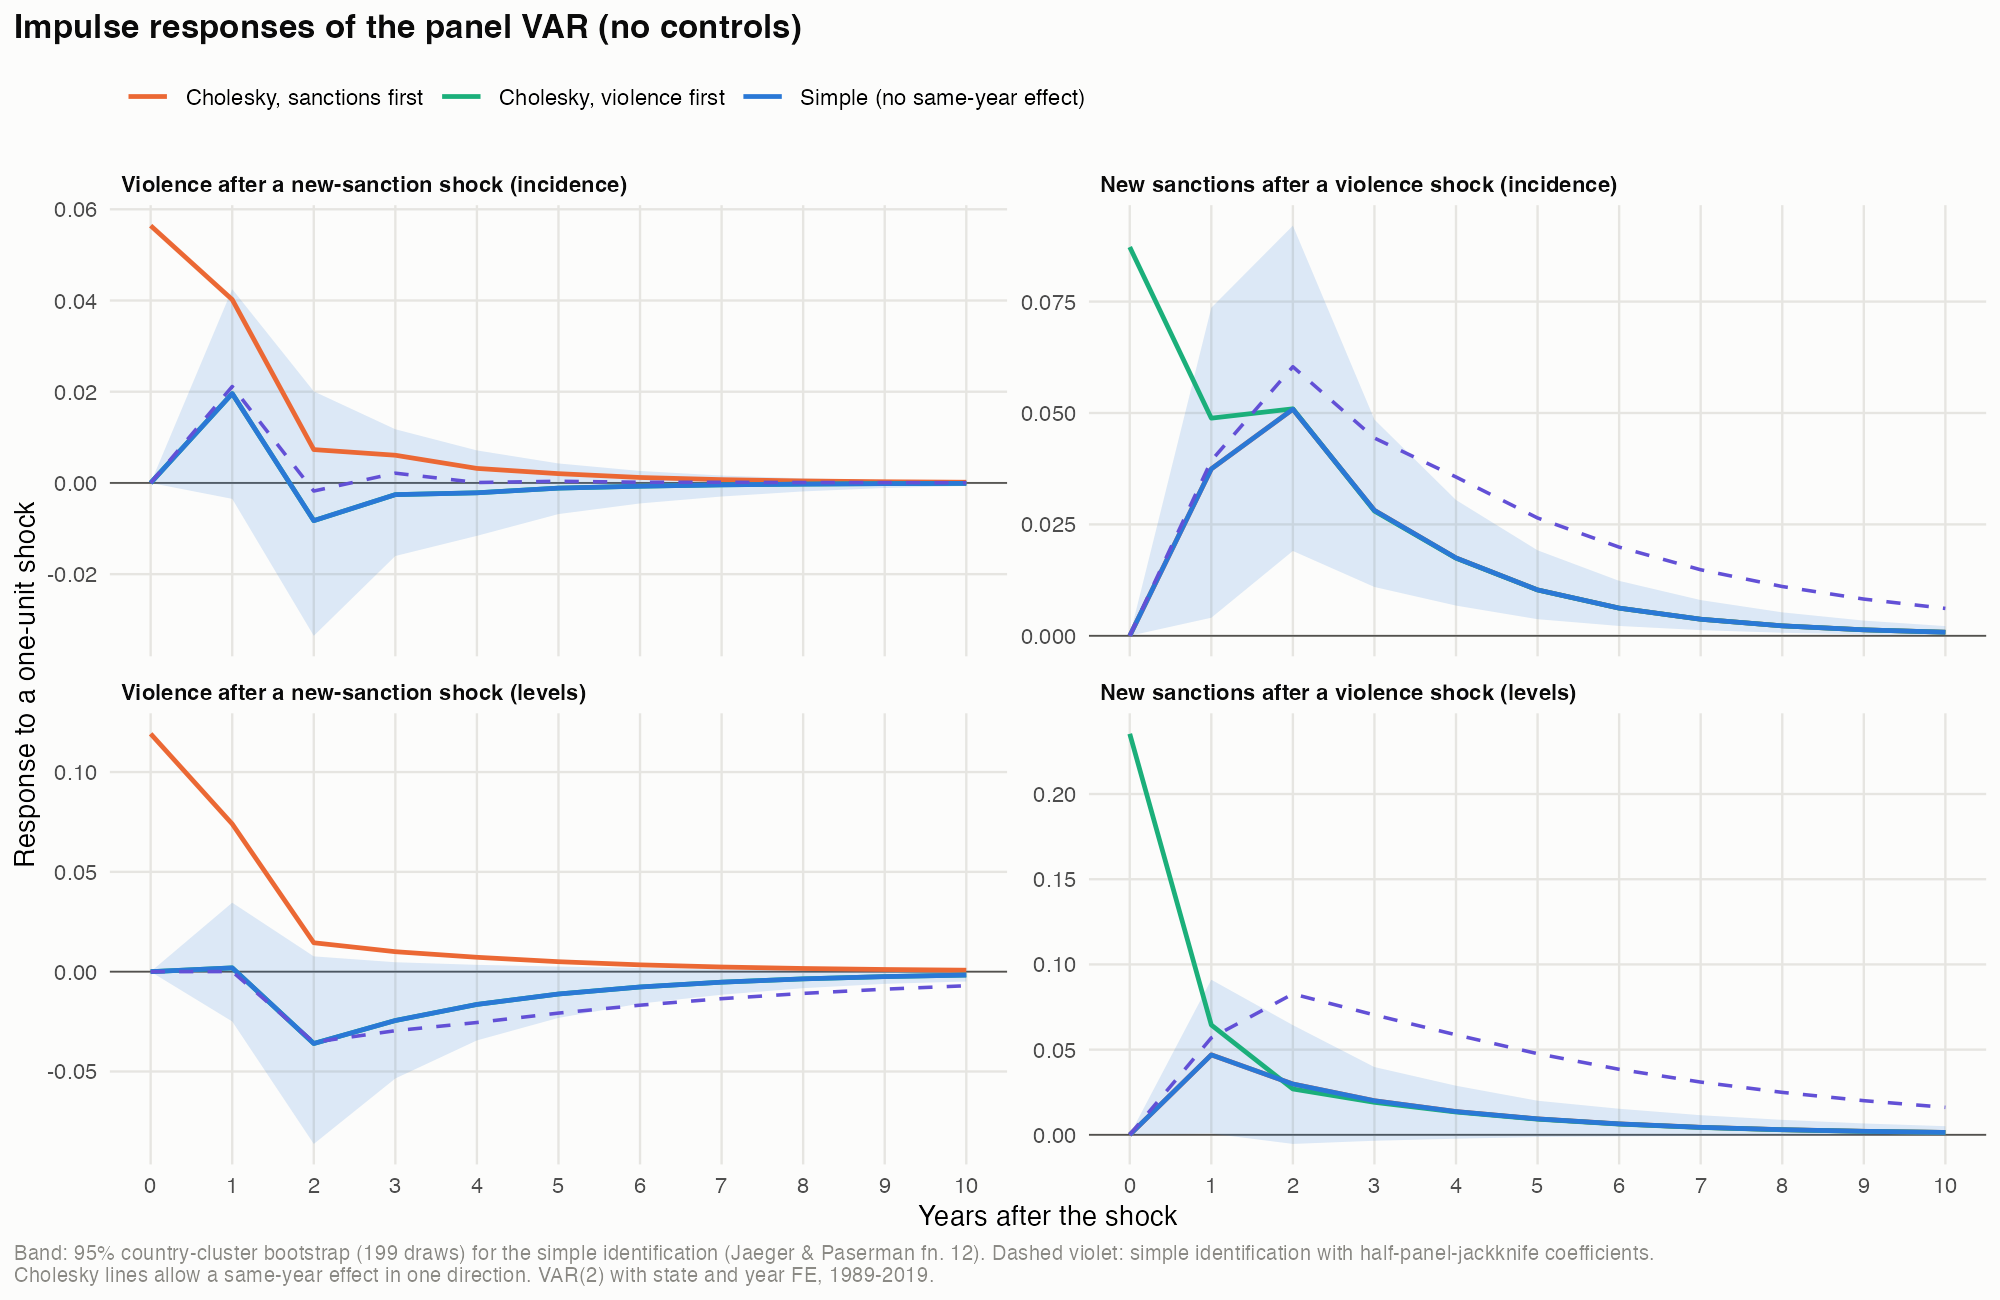
\includegraphics[width=\textwidth]{fig12_irf_no_controls.png}
\caption{Impulse responses, VAR without controls}
\label{fig:irfnocontrols}
\end{figure}

\begin{figure}[htbp]
\centering
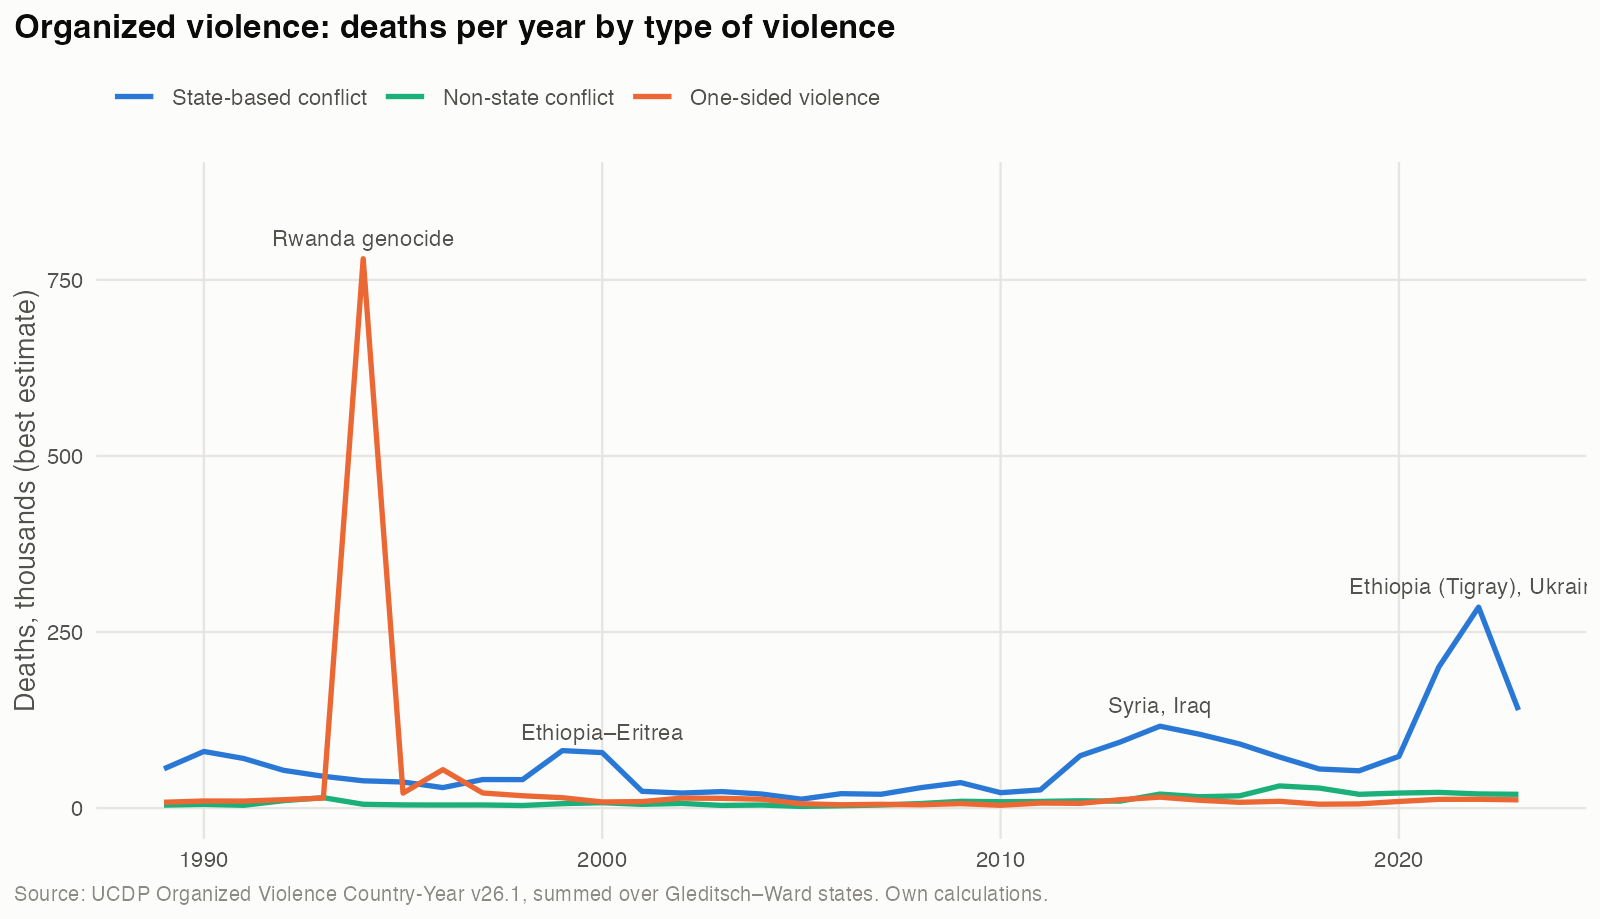
\includegraphics[width=0.85\textwidth]{fig3_violence_deaths_by_type.png}
\caption{Deaths in organized violence by type (UCDP)}
\label{fig:deaths}
\end{figure}

\end{document}
